%% LyX 2.2.0 created this file.  For more info, see http://www.lyx.org/.
%% Do not edit unless you really know what you are doing.
\documentclass[english]{article}
\usepackage[T1]{fontenc}
\usepackage[latin9]{inputenc}
\synctex=1
\usepackage{babel}
\usepackage{array}
\usepackage{varioref}
\usepackage{textcomp}
\usepackage{url}
\usepackage{multirow}
\usepackage{tipa}
\usepackage{amsmath}
\usepackage{amsthm}
\usepackage{amssymb}
\usepackage{graphicx}
\usepackage[unicode=true,
 bookmarks=true,bookmarksnumbered=false,bookmarksopen=false,
 breaklinks=false,pdfborder={0 0 1},backref=false,colorlinks=false]
 {hyperref}
\hypersetup{pdftitle={Computability, Complexity, and Algorithms Course Notes},
 pdfauthor={Brandon A. Durepo},
 pdfkeywords={Algorithms, Automata, Computabilty, Complexity, Analysis}}

\makeatletter

%%%%%%%%%%%%%%%%%%%%%%%%%%%%%% LyX specific LaTeX commands.
%% Because html converters don't know tabularnewline
\providecommand{\tabularnewline}{\\}

%%%%%%%%%%%%%%%%%%%%%%%%%%%%%% Textclass specific LaTeX commands.
  \theoremstyle{definition}
  \newtheorem*{example*}{\protect\examplename}
\theoremstyle{plain}
\newtheorem{thm}{\protect\theoremname}
  \theoremstyle{definition}
  \newtheorem{example}[thm]{\protect\examplename}
  \theoremstyle{definition}
  \newtheorem*{sol*}{\protect\solutionname}
  \theoremstyle{plain}
  \newtheorem{cor}[thm]{\protect\corollaryname}
  \theoremstyle{remark}
  \newtheorem{claim}[thm]{\protect\claimname}
  \theoremstyle{plain}
  \newtheorem{lem}[thm]{\protect\lemmaname}

\@ifundefined{date}{}{\date{}}
\makeatother

  \providecommand{\claimname}{Claim}
  \providecommand{\corollaryname}{Corollary}
  \providecommand{\examplename}{Example}
  \providecommand{\lemmaname}{Lemma}
  \providecommand{\solutionname}{Solution}
\providecommand{\theoremname}{Theorem}

\begin{document}
\begin{figure}
\centering{}\includegraphics[scale=0.25]{Pictures/techTower}\caption{Tech Tower was built in 1888, and it is the oldest surviving building
on campus. Names of past alumi are scrawled on the inside of the bell
tower dating back to the earliest classes.}
\end{figure}


\title{Notes on Computability, Complexity, and Algorithms}

\author{Brandon A. Durepo}

\maketitle
\pagebreak{}
\begin{quote}
\begin{flushright}
``Sapere aude.'' \textendash{} Horace
\par\end{flushright}

\end{quote}
\tableofcontents{}

\section*{Preface}

The purpose of this document is to help students of all stripes succeed
in Georgia Tech's course on Computability, Complexity and Algorithms
more formally known as CS6505. It is no secret that this class is
a humdinger. Many students find this course to be challenging and
the topics can be opaque at times to the newcomer. However with grit,
determination, and luck you, the reader, can reap the many benefits
that this course offers. 

In following sections I outline some of the key concepts you will
need to be successful in the course. I make no assumptions about prerequisite
knowledge and attempt to provide you the green-field perspective on
the subject matter. In many cases, if you have already seen the information
it is safe to skip forward and not concern yourself what may be obvious
to you, but I encourage you to read all the sections because additional
clarity may be gained with another pass.

\part{Mathematics and Logic}

\section{Discrete Mathematics}

\begin{figure}
\begin{centering}
\begin{tabular}{|c|c|}
\hline 
Equivalence & Name\tabularnewline
\hline 
\hline 
$p\land T\equiv p$, $p\lor F\equiv F$ & Identity Laws\tabularnewline
\hline 
$p\lor T\equiv T$, $p\land F\equiv F$ & Domination Laws\tabularnewline
\hline 
$p\lor p\equiv p$, $p\land p\equiv p$ & Idempotent Laws\tabularnewline
\hline 
$\lnot(\lnot p)\equiv p$ & Double Negation Laws\tabularnewline
\hline 
$p\lor q\equiv q\lor p$, $p\land q\equiv q\land p$ & Communicative Laws\tabularnewline
\hline 
$(p\lor q)\lor r\equiv p\lor(q\lor r)$, $(p\land q)\land r\equiv p\land(q\land r)$ & Associative Laws\tabularnewline
\hline 
$p\lor(q\land r)\equiv(p\lor q)\land(p\lor r)$, $p\land(q\lor r)\equiv(p\land q)\lor(p\land r)$ & Distributive Laws\tabularnewline
\hline 
$\lnot(p\land q)\equiv\lnot p\lor\lnot q$, $\lnot(p\lor q)\equiv\lnot p\land\lnot q$ & De Morgan's Law\tabularnewline
\hline 
$p\lor(p\land q)\equiv p$, $p\land(p\lor q)\equiv p$ & Absoption Law\tabularnewline
\hline 
$p\lor\lnot p\equiv T$, $p\land\lnot p\equiv F$ & Negation Laws\tabularnewline
\hline 
\end{tabular} %
\begin{tabular}{|c|}
\hline 
Logical Equivalences Involving Conditional Statements\tabularnewline
\hline 
\hline 
$p\rightarrow q\equiv\lnot p\lor q\equiv\lnot q\rightarrow\lnot p$\tabularnewline
\hline 
$p\lor q\equiv\lnot p\rightarrow q$\tabularnewline
\hline 
$p\land q\equiv\lnot(p\rightarrow\lnot q)$\tabularnewline
\hline 
$\lnot(p\rightarrow q)\equiv p\land\lnot q$\tabularnewline
\hline 
$(p\rightarrow q)\land(p\rightarrow r)\equiv p\rightarrow(q\land r)$\tabularnewline
\hline 
$(p\rightarrow r)\land(q\rightarrow r)\equiv(p\lor q)\rightarrow r$\tabularnewline
\hline 
$(p\rightarrow q)\lor(p\rightarrow r)\equiv p\rightarrow(q\lor r)$\tabularnewline
\hline 
$(p\rightarrow r)\lor(q\rightarrow r)\equiv(p\land q)\rightarrow r$\tabularnewline
\hline 
\end{tabular} %
\begin{tabular}{|c|}
\hline 
Logical Equivalences Involving Biconditional Statements\tabularnewline
\hline 
\hline 
$p\leftrightarrow q\equiv(p\rightarrow q)\land(q\rightarrow p)$\tabularnewline
\hline 
$p\leftrightarrow q\equiv\lnot p\leftrightarrow\lnot q$\tabularnewline
\hline 
$p\leftrightarrow q\equiv(p\land q)\lor(\lnot p\land\lnot q)\lor(\lnot p\land\lnot q)$\tabularnewline
\hline 
$\lnot(p\leftrightarrow q)\equiv p\leftrightarrow\lnot q$\tabularnewline
\hline 
\end{tabular}
\par\end{centering}
\caption{\label{fig:lawsOfLogic} Logical equivalences. Idempotent denotes
an element of a set that is unchanged in value when multiplied or
otherwise operated on by itself.}
\end{figure}


\subsection{Propositional and Sentential Logic\label{sec:propositionalSententialLogic}}

All logical expressions can be described in some combination of \emph{logical
operators} and \emph{implications}. The logical operators consist
of the following: the logical conjunction $\land$, the logical disjunction
$\lor$, and the negation $\lnot$. The implication is made up of
two propositional variables $p$and $q.$ $p$is often called the
\emph{premise} or \emph{hypothesis} or \emph{antecedent}, while $q$may
be referred to as the \emph{conclusion}, or \emph{consequence}. Truth
tables are a way of tabulating the values of arbitrary logical expressions
by enumerating all possible truth values for the component of the
expressions. The usefulness of this technique quickly diminishes as
the number of proposition variables goes beyond 4. In this case the
number of rows in the truth table is $2^{4}=16$. The precedence of
logical operators is negation, conjunction, disjunction.

The implication is given by the symbol $\rightarrow$. Variations
on the traditional implication of $p\rightarrow q$ include its \emph{converse}
$q\rightarrow p$, the \emph{contraposative} $\lnot q\rightarrow\lnot p$,
and the \emph{inverse} $\lnot p\rightarrow\lnot q$. A biconditional
or implication statement is a slightly more creative way to use the
implication. A table of logical equivalences is provided in Figure\vref{fig:lawsOfLogic}.

Use of these laws can allow you to establish an equivalence of complex
propositional statements with a more distilled simplified version.
Propositional statements are said to be \emph{satisfiable} if some
combination of truth assignments to the propositional variables makes
the statement true.

\subsection{Predicate Calculus and Quantification Logic}

Predicate logic is a generalization of propositional logic onto arbitrary
statements. \emph{Propositional functions} given by a capital letter
and a number of parameters are used to define propositional statements.
An example, ``Computer $x$, is functioning properly'' would be
written as $P(x).$ 

Quantification expresses the extent to which a predicate is true over
a range of elements. In English, the words all, some, many, none,
and few are used in quantification's. The \emph{universal quantification}
symbol for all is given by $\forall$. The \emph{existential quantification}
symbol for exists is $\exists$. The statement $\forall xP(x)$ reads
``For all computers given by $x$, computer $x$is functioning properly.''
If there is a single instance of a universal variable which is false
then the predicate becomes false. If for all instances of an existential
variables the value is false then the statement is false. Quantification
operators have higher precedence than logical operators. Predicates
used with quantifiers are said to be \emph{bound variables} while
those without are said to be \emph{free variables}.

\begin{figure}
\begin{centering}
\begin{tabular}{|c|}
\hline 
$\lnot\forall xP(x)\equiv\exists x\lnot P(x).$\tabularnewline
\hline 
$\lnot\exists xP(x)\equiv\forall\lnot P($x).\tabularnewline
\hline 
\end{tabular}
\par\end{centering}
\caption{\label{fig:quantificationNegation} This table shows the equivalence
relations on predicates with quantification symbols.}

\end{figure}


\subsection{Rules of Inference}

The \emph{validity} of a proofs arguments are derived from the truth
of the premises it offers. An argument in propositional logic is a
sequence of propositions. All but the final proposition in the argument
are called \emph{premises} and the final proposition is called the
\emph{conclusion}. An argument is valid if the truth of all its premises
implies that the conclusion is true. An argument form in propositional
logic is a sequence of compound propositions involving \emph{propositional
variables}. 

An argument's form is valid no matter which particular propositions
are substituted for the propositional variables in its premises, the
conclusion is true if the premises are all true. The rules of inference
provide the templates of logical propositions which, when given in
a valid combination, yield valid arguments. The rules are given in
Figure\vref{fig:inferenceRules}. Additionally, the Rules of Inference
applies to quantification logic as well as shown in the table.

\begin{figure}
\begin{centering}
\begin{tabular}{|c|c|}
\hline 
Tautology & Name\tabularnewline
\hline 
\hline 
$(p\land(p\rightarrow q))\rightarrow q$ & Modus ponens\tabularnewline
\hline 
$(\neg q\land(p\rightarrow q))\rightarrow q$ & Modus tollens\tabularnewline
\hline 
$((p\rightarrow q)\land(q\rightarrow r))\rightarrow(p\rightarrow r)$ & Hypothetical syllogism\tabularnewline
\hline 
$((p\lor q)\land\neg p)\rightarrow q$ & Disjunctive syllogism\tabularnewline
\hline 
$p\rightarrow(p\lor q)$ & Addition\tabularnewline
\hline 
$(p\land q)\rightarrow q$ & Simplification\tabularnewline
\hline 
$((p)\land(q))\rightarrow(p\land q)$ & Conjunction\tabularnewline
\hline 
$(p\lor q)\land(\neg p\lor r)\rightarrow(q\lor r)$ & Resolution\tabularnewline
\hline 
\end{tabular}
\par\end{centering}
\begin{centering}
\begin{tabular}{|c|c|}
\hline 
Inference Rule & Name\tabularnewline
\hline 
\hline 
$\frac{\forall xP(x)}{\therefore P(c)}$ & Universal instantiation\tabularnewline
\hline 
$\frac{P(c)}{\therefore\forall xP(x)}$ for an arbitrary $c$ & Universal generalization\tabularnewline
\hline 
$\frac{\exists xP(x)}{\therefore P(c)}$ for some element $c$ & Existential instantiation\tabularnewline
\hline 
$\frac{P(c)}{\therefore\exists xP(x)}$ & Existential generalization\tabularnewline
\hline 
\end{tabular}
\par\end{centering}
\caption{\label{fig:inferenceRules}This table gives the Rules of Inference.}
\end{figure}


\subsection{Proofs}

In order to begin to understand how to construct valid proof it is
important to understand the terminology that is used. 

\subsubsection{Terminology of Proofs}
\begin{itemize}
\item a \emph{theorem} is a statement that can be shown to be true.
\item A \emph{proof} is a valid argument that establishes the truth of a
theorem.
\item \emph{axioms} (or \emph{postulates}) are statements we assume to be
true.
\item A \emph{lemma} is a less important theorem that is helpful in the
proof of other results.
\item A \emph{corollary} is a theorem that can be established directly from
a theorem that has been proved.
\item \emph{without loss of generality} (WLOG) means that the author of
a proof is omitting the proof of one of the cases in a proof by cases.
\end{itemize}

\subsubsection{Types of Proofs}
\begin{itemize}
\item \emph{Direct Proofs} is a proof that assumes the antecedent of the
implication is true and seeks to justify and prove the conclusion
of the theorem by examining the characteristics of the relationship
of the antecedent and conclusion. A direct proof may use axioms, definitions,
and previously proven theorems, together with rules of inference,
to show that q must also be true. Here we are establishing the truth
of the proof based on row 1 of the truth table found in Figure\vref{fig:implicationTruthTable}.
\end{itemize}
\begin{figure}
\begin{centering}
\begin{tabular}{|c|c|c|}
\hline 
$p$ & $q$ & $p\rightarrow q$\tabularnewline
\hline 
\hline 
T & T & T\tabularnewline
\hline 
T & F & F\tabularnewline
\hline 
F & T & T\tabularnewline
\hline 
F & F & T\tabularnewline
\hline 
\end{tabular} %
\begin{tabular}{|c|c|c|}
\hline 
$p$ & $q$ & $\neg q\rightarrow\neg p$\tabularnewline
\hline 
\hline 
T & T & T\tabularnewline
\hline 
T & F & F\tabularnewline
\hline 
F & T & T\tabularnewline
\hline 
F & F & T\tabularnewline
\hline 
\end{tabular}
\par\end{centering}
\caption{\label{fig:implicationTruthTable} Truth table for the implication
and its contraposative.}
\end{figure}

\begin{itemize}
\item In juxtaposition to the direct proof we have the indirect proof techniques.
Indirect proofs do not start with the assumption of the truth of the
premise to derive the truth of the conclusion. The\emph{ Proof by
Contraposition }technique takes advantage of the equivalence of the
contrapostion of the implication to prove the conclusion. That is,
$\neg q\rightarrow\neg p\equiv p\rightarrow q$ as shown in Figure\vref{fig:lawsOfLogic}.
The template for this type of proof is constructed by assuming the
conclusion $q$is false which implies that the premise $p$ is also
false. 
\item The trivial and vacuous proofs strategies are the simplest strategies.
A \emph{Trivial Proof} is a proof that derives the truth of the conclusion
based on the fact that the premise is false. This logic is based on
row 3 of the implication truth table. A Vacuous Proof is a proof based
on the fact the conclusion is true also show in row 3.
\item \emph{Proofs by Contradiction }seek to find a contradictory conclusion
$q=r\land\neg r$, such that $\neg p\rightarrow q$ is true. We must
show that $p$is true by showing $\neg p$ is false so that we can
target row 4 in the implication truth table. 
\item \emph{Proofs of Equivalence }To prove a theorem that is a biconditional
statement, that is, a statement of the form $p\leftrightarrow q$,
we show that $p\rightarrow q$ and $q\rightarrow p$. The validity
of this approach is based on the tautology $(p\leftrightarrow q)\equiv(p\rightarrow q)\land(q\rightarrow p)$
\item \emph{Proofs by Counterexample }in this type of proof we typically
try to debunk the truth of a universal quantifier over some predicate.
If we find one instance is false, then we can conclude the predicate
is false\emph{.}
\item \emph{Proof by Cases and the Exhaustive Proof }sometimes using a single
argument to cover the premise of a proof is not sufficient. As an
alternative, we can devises cases that cover the entire domain of
the proof and address each case in turn to prove the conclusion. This
proof technique relies on the following tautology.
\[
[(p_{1}\lor p_{2}\lor\ldots\lor p_{n})\rightarrow q]\leftrightarrow[(p_{1}\rightarrow q)\land(p_{2}\rightarrow q)\land\ldots\land(p_{n}\rightarrow q)]
\]
\item \emph{Existence Proofs }a proof of this type is of the form $\exists xP(x)$.
This type of proof can be proven by providing a \emph{witness} $a,$
a instance of $x$where $P(a)$ is true. This type of strategy is
called a \emph{constructive} proof. A nonconstructive existence uses
some other means to prove that $\exists xP(x)$. Often contradiction
is used.
\item \emph{Uniqueness Proofs }in this type of proof we show that a unique
element with a particular property exists. These types of proofs are
composed of two steps. First you must prove the existence of the element.
Then we show that if $y\neq x$, then $y$does not have the particular
property of $x.$ Formally, uniqueness proofs are of the form:
\[
\exists x(P(x)\land\forall y(y\neq x\rightarrow\neg P(y))).
\]
\end{itemize}
\begin{figure}
\begin{centering}
\begin{tabular}{|c|c|}
\hline 
Direct Methods & Indirect Methods\tabularnewline
\hline 
\hline 
Direct Proof & Proof by Contraposition\tabularnewline
\hline 
Proof by Cases & Proof by Contradiction\tabularnewline
\hline 
Exhaustive Proof & Proof by Counterexample\tabularnewline
\hline 
Existence Proof & \tabularnewline
\hline 
Uniqueness Proof & \tabularnewline
\hline 
\end{tabular}
\par\end{centering}
\caption{Classification of the proof strategies}

\end{figure}


\subsubsection{Strategies for Constructing Proofs}

The following general approach for constructing proofs is often helpful.
\begin{enumerate}
\item Replace terms by their definitions.
\item Analyze the hypothesis and conclusion.
\item Attempt to construct the proof using the direct proof method, if the
statement is a conditional statement.
\begin{enumerate}
\item If you fail to construct a direct proof, attempt to provide an indirect
proof.
\item If both the direct and indirect proof methods don't work, then attempt
a proof by contradiction.
\end{enumerate}
\end{enumerate}
\emph{Forward reasoning} as well as\emph{ backward reasoning} is necessary
to construct valid proofs. Forward reasoning uses premises as well
as previously proven theorems and axioms to prove the conclusion.
In a direct proof this is the method of choice. Indirect proofs often
will often require backward reasoning. In backward reasoning we attempt
to find a statement $p$that we can prove true with $p\rightarrow q.$

\emph{Adaptation }of existing proofs is often a fruitful procedure.
Even if the final conclusions required are not the same, it may be
constructive to look to the previous proves for ideas which may help
in your new proof.

\subsection{Mathematical Structures: Sets, Sequences, Series, and Matrices\label{sec:Sets}}

Mathematical structures are the foundation on which reasoning is carried
out. In the following sections we cover sets, sequences, series and
matricies.

\subsubsection{Sets}

A \emph{set} is an unordered collection of objects. A object is said
to be \emph{contained} within a set when it is a member of the set.
The epsilon symbol is used to denote membership in a set ( object
$a$is in set $A$ is written $a\epsilon A$). A strikethrough on
the episilon symbol means that the object is not a member of the set.

Uppercase English letters traditionally denote the names of sets,
while lowercase English letters represents objects of a set. Sets
may be described by the \emph{roster method }which lists all the elements
of the set explicitly surrounded by curly braces, or by using a \emph{set
former} sometimes called \emph{set builder}. A set former works by
specifing a variable that represents a member of the set followed
by the characteristics of the variable. Often the name of the variable
and the characteristics are seperated by a vertical bar or colon which
should be read ``such that.''
\begin{example*}
$EQTM$=\{($M_{1}$,$M_{2}$) | $L(M_{1})=L(M_{2})\}$. This set former
describes the set of pairs of Turing machines that have the same language.
\end{example*}
Often set formers will reference equivalance classes from number theory
such as the rational numbers etc. A list of importance number classes
is given below. These special sets are denoted by a special script
font that distinquishes them from other sets.
\begin{itemize}
\item $\mathbb{N}=\{0,1,2,\ldots\}$. The set of natural numbers. Some regard
0 as a natural number, others do not. Be sure to ask if there is any
question.
\item $\mathbb{Z}=\{\ldots,-2,-1,0,1,2,\ldots\}$. The set of integers.
The positive or negative superscript denotes the positve or negative
subset of the integers. $\mathbb{Z}^{+}\subset\mathbb{Z},\mathbb{Z}^{-}\subset\mathbb{Z}$
\item $\mathbb{Q=}$\{$\frac{p}{q}:p\epsilon\mathbb{Z}\land q\epsilon\mathbb{Z},q\neq0\}$.
The set of rational numbers such that each is represented as a ratio
of integers.
\item $\mathbb{R}$ the set of real numbers, or the set of positive real
numbers $\mathbb{R}^{+}$.
\item $\mathbb{C}$ the set of complex numbers.
\end{itemize}
It is important to note the relationship amongst these sets. The diagram
in Figure\ref{fig:numberClassification} is a good reference for reasoning
about the relationships which comes in hany for writing proofs.

Some other terminology often used includes the \emph{empty set }or
a \emph{null set} which means a set of no elements. It is denoted
by the symbol $\emptyset$. A \emph{singleton set} is a name for a
set with a single element. A set is said to be a \emph{subset} if
and only if every element of one set is also a member of the another
set. The subset relationship represented by the symbol $\subseteq$.
When we want to say that a set is a subset of another set, not necesarilly
equivalent we use the proper subset symbol $\subset$.

Sets $A$ and $B$ are said to be equivalant if $A\subseteq B$ and
$B\subseteq A$, and the size of set is called its \emph{cardinality.
}Cardinality is denoted by vertical bars surrounding the set name.

The \emph{power set} of a set gives all combinations of subsets of
a given set, and it is denoted as $2^{S}$ or $\mathcal{P}(S)$ where
S is the set under consideration.
\begin{example*}
The powerset of $S=\{a,b,c\}$ $\mathcal{P}(S)=\{\emptyset,\{a\},\{b\},\{c\},\{a,b\},\{a,c\},\{b,c\},\{a,b,c\}\}$ 
\end{example*}
The Cartesian product or Cross product of two sets denoted by $A\times B$
(read ``A cross B'') is the set of ordered n-tuples $(a_{i},b_{j})$
for $i\leq|A|$ and $j\leq|B|$. In more general terms the Cartesian
product of the sets $A_{1},A_{2},\ldots,A_{n}$ denoted by $A_{1}\times A_{2}\times\ldots\times A_{n}$
is the set of ordered n-tuples $(a_{1},a_{2},\ldots,a_{n})$, where
$a_{i}$ belongs to $Ai$ for $1\leq i\leq n$. 

The \emph{union} of the sets $A$ and $B$, denoted by $A\bigcup B$,
is the set that contains those elements that are either in A or in
B, or in both. Let A and B be sets. The \emph{intersection} of the
sets $A$ and $B$, denoted by $A\bigcap B$, is the set containing
those elements in both $A$ and $B$. Two sets are called \emph{disjoint}
if their intersection is the empty set. The \emph{complement} of the
set $A$. denoted by $\bar{A}$, is the complement of $A$ with respect
to $U$. Therefore, the complement of the set $A$ is $U-A$. An illustration
of the aforementioned set operations is given in figure below. A table
of important set identities is given in Figure\vref{fig:setIdentites}.

\begin{figure}
\begin{centering}
\begin{tabular}{|c|c|}
\hline 
Identity & Name\tabularnewline
\hline 
$A\bigcap U=A$ $A\bigcup\emptyset=A$ & Identity laws\tabularnewline
\hline 
$A\bigcup U=U$$A\bigcap\emptyset=\emptyset$ & Domination laws\tabularnewline
\hline 
$A\bigcup A=A$ $A\bigcap A=A$ & Idempotent laws\tabularnewline
\hline 
$\overline{(\overline{A})}=A$ & Complementation law\tabularnewline
\hline 
$A\bigcup B=B\bigcup A$ $A\bigcap B=B\bigcap A$ & Communative laws\tabularnewline
\hline 
$A\bigcup(B\bigcup C)=(A\bigcup B)\bigcup C$ $A\bigcap(B\bigcap C)=(A\bigcap B)\bigcap C$ & Associative laws\tabularnewline
\hline 
$A\bigcup(B\bigcap C)=(A\bigcup B)\bigcap(A\bigcup C)$ $A\bigcap(B\bigcup C)=(A\bigcap B)\bigcup(A\bigcap C)$ & Distributive laws\tabularnewline
\hline 
$\overline{A\bigcap B}=\bar{A}\bigcup\bar{B}$ $\overline{A\bigcup B}=\bar{A}\bigcap\bar{B}$ & De Morgan's laws\tabularnewline
\hline 
$A\bigcup(A\bigcap B)=A$ $A\bigcap(A\bigcup B)=A$ & Absorption laws\tabularnewline
\hline 
$A\bigcup\bar{A}=U$ $A\bigcap\bar{A}=\emptyset$ & Complement laws\tabularnewline
\hline 
\end{tabular}
\par\end{centering}
\caption{\label{fig:setIdentites}The table lists important set identites.
Refer to these when writing proofs.}

\end{figure}

\begin{figure}
\begin{centering}
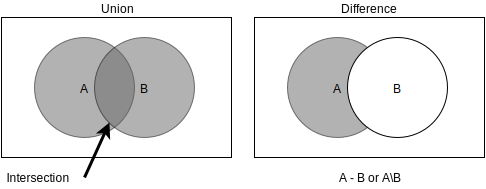
\includegraphics[scale=0.5]{Diagrams/setOperations}
\par\end{centering}
\caption{\label{fig:setOperations}The intersection is given by the darkly
shaded region. The union is given by all the shaded regions in the
left-most figure. This figure demonstrates the idea that elements
of the union count the elements of the intersection twice. The difference
is given by the right-most figure. The intersection is equivalent
to $A\bigcap\bar{B}$.}
\end{figure}

Understanding countability of sets is critical. The notion of counting
as it pertains to counting in sets is called a sets cardinality. As
we have seen in previous sections sets may be finite or infinite.
In the case of infinite sets the notion of counting to infinity seems
rather abstract. In fact, the notion of infinity is not unique in
itself there are infinities that are countable and those that are
uncountable. Mathematicians refer to these ideas as \emph{countably
infinte} and \emph{uncountably infinite}.

The sets $A$ and $B$ have the same cardinality if and only if there
is a \emph{one-to-one correspondence} from $A$ to $B$. When $A$
and $B$ have the same cardinality, we write $|A|=|B|$. When we apply
this definition to finite sets it seems quite intuitive, however when
applying this definition to an infinite set a novice students will
be quite perplexed. Cardinality as it applies to infinite sets informs
us of the relative size of sets under consideration. The purpose of
a correspondence function is to establish some footing as to the relative
size of one set versus another. 

If there is a \emph{one-to-one} function from $A$ to $B$, the cardinality
of $A$ is less than or the same as the cardinality of $B$ and we
write $|A|\leq|B|$. Moreover, when $|A|\leq|B|$ and $A$ and $B$
have different cardinality, we say that the cardinality of $A$ is
less than the cardinality of $B$ and we write $|A|<|B|$.
\begin{itemize}
\item A set that is either finite or has the same cardinality as the set
of positive integers is called \emph{countable}. A set that is not
countable is called \emph{uncountable}.When an infinite set $S$ is
countable, we denote the cardinality of S by $\aleph_{0}$ (where
$\aleph$ is aleph, the first letter of the Hebrew alphabet, pronounced
'\textscripta \textlengthmark l\textepsilon f''). We write $|S|=\aleph_{0}$.
\end{itemize}
\textbf{Hilbert's Grand Hotel} is classical example of the principles
of countablility. Hilbert's Grand Hotel is a hotel with a countably
infinite number of rooms such that the hotel when fully occupied by
guests can accomadate a finitely many number of new guests or a countably
infinite number of new guests without evicting any current tenants
(quite a bizzare notion).

The Sch�der-Bernstein Theorem states that if $A$ and $B$ are sets
with $|A|\le|B|$ and $|B|\le|A|$, then $|A|=|B|$. In other words,
if there are one-to-one functions $f$ from $A$ to $B$ and $g$
from $B$ to $A$, then there is a one-to-one correspondence between
$A$ and $B$. Rosen refers us to Velleman for a proof of this theorem.

The Continuum Hypothesis 

\subsubsection{Sequences and Summations}

A sequence is a function from a subset of the set of integers (usually
either the set $\{0,1,2,\ldots\}$or the set $\{1,2,3,\ldots\}$)
to a set S. We use the notation $a_{n}$ to denote the image of the
integer $n$. We call $a_{n}$a term of the sequence. \href{https://oeis.org/}{The Online Encyclopedia of Integer Sequences}
is a useful source for getting background information on notable integer
sequences.

\begin{figure}
\begin{centering}
\begin{tabular}{|c|c|}
\hline 
Summations & Closed Form\tabularnewline
\hline 
\hline 
$\sum_{k=0}^{n}ar^{k},(r\neq0)$ & $\frac{ar^{n+1}-a}{r-1},r\neq1$\tabularnewline
\hline 
$\sum_{k=1}^{n}k$ & $\frac{n(n+1)}{2}$\tabularnewline
\hline 
$\sum_{k=1}^{n}k^{2}$ & $\frac{n(n+1)(2n+1)}{6}$\tabularnewline
\hline 
$\sum_{k=1}^{n}k^{3}$ & $\frac{n^{2}(n+1)^{2}}{4}$\tabularnewline
\hline 
$\sum_{k=0}^{\infty}x^{k},|x|<1$ & $\frac{1}{1-x},x\neq1$\tabularnewline
\hline 
$\sum_{k=1}^{\infty}kx^{k-1},|x|<1$ & $\frac{1}{(1-x)^{2}}$\tabularnewline
\hline 
\end{tabular}
\par\end{centering}
\caption{\label{fig:usefulSums}Rosen provides a table of useful sums.}

\end{figure}


\subsection{Relations\label{sec:Relations}}

\subsection{Functions\label{sec:Functions}}

A \emph{function} (sometimes called a \emph{mapping} or \emph{transformation})
\emph{$f$ }from $A$ to $B$ is an assignment of exactly one element
of $B$ to each element of $A$. We write $f(a)=b$ if $b$ is the
unique element of $B$ assigned by the function $f$ to the element
$a$of $A$.

If $f$is a function from $A$ to $B,$we writed $f:A\rightarrow B$.
If $f$ is a function from $A$ to $B$, we say that $A$ is the domain
of $f$and $B$ is the codomain of $f$. If $f(a)=b$, we say that
b is the image of $a$and $a$is a preminage of $b$. The \emph{range
}, or \emph{image,} of $f$ is the set of all images of elements of
$A$. Also, if $f$ is a function from $A$ to $B$, we say htat $f$
\emph{maps $A$ to $B$. }The range is a subset of the codomain, and
the image is a memeber of the range.

\subsubsection{One-to-One and Onto Functions and Their Nature}

Given sets $A$ and $B,$ a function $f$ is said to be \emph{one-to-one,
}or \emph{injuction}, if and only if $f(a)=f(b)$ imples that $a=b$
for all $a$and $b$ in the domain of $f$. A function is said to
be \emph{injective }if it is one-to-one. A function is injecitve if
and only if it takes on different images for all elements in its domain.
Figure\vref{fig:classesOfFunctions} shows examples of each combination
of function and a description as to why they are classified as such.

A function $f$ from $A$ to $B$ is called \emph{onto, }or a \emph{surjection,
}if and only if\emph{ }for every element $b\epsilon B$ there is an
element $a\epsilon A$ with $f(a)=b$. A function $f$ is called surjective
if it is onto. The function $f$ is a \emph{one-to-one correspondence},
or a \emph{bijection}, if it is surjective and injective. A function
of this type is called \emph{bijective}. Visually, this is shown in
Figure

\begin{figure}
\begin{centering}
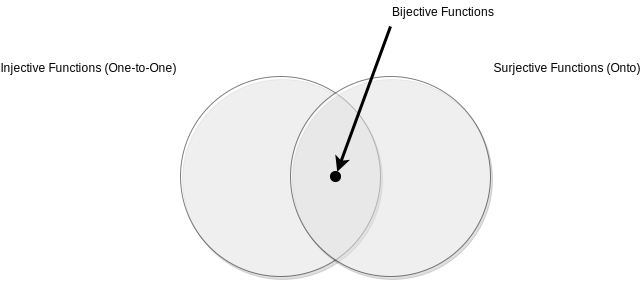
\includegraphics[scale=0.5]{Diagrams/visualizeFunctionClasses}
\par\end{centering}
\caption{\label{fig:visualizeFunctionClasses}Bijective functions are in the
intersection fo the Injective and Surjective functions.}

\end{figure}

A function $f$ whose domain and codomain are subsets of the set of
real numbeers is called \emph{increasing} if $f(k)\leq f(k+1)$, and
\emph{strictly increading} if $f(k)<f(k+1)$. Similiarly, $f$ is
\emph{decreaseing} if $f(k)\geq f(k+1)$, and \emph{strictly decreasing
}if $f(k)>f(k+1)$.

\begin{figure}
\begin{centering}
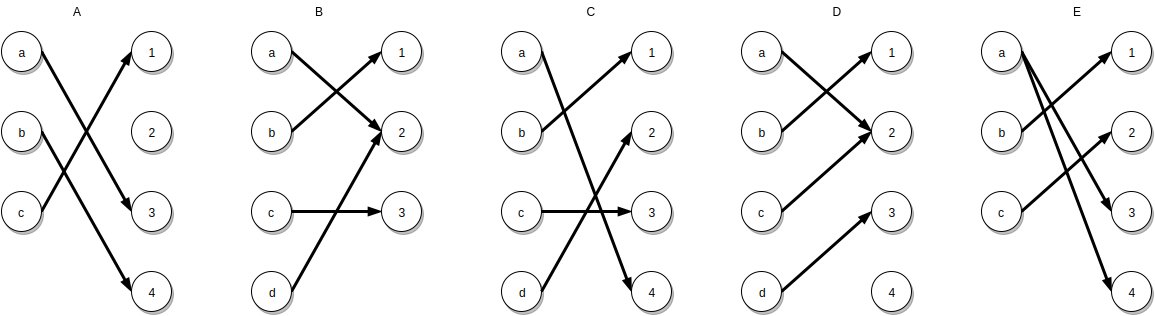
\includegraphics[scale=0.3]{Diagrams/ClassesOfFunctions}
\par\end{centering}
\caption{\label{fig:classesOfFunctions} A) The function given by this figure
is injective because elements of the range map to distinct elements
of the domain. However, it is not surjective because not all elements
of the range have a corresponding element in the range. Namely, $2$
is not mapped to an element of the domain. B) The function given by
this figure is surjective because every element in the range has been
mapped. However, it is not injective because the mapping is not distinct.
Both $a$and $d$ of the domain map to $2$ in the range. C) The function
given by this figure is both injective and surjective, and therefore
it is a bijection. D) This figure does not model a function that is
eigher a injective or surjective, and therefore it is not a bijection.
D) This figure violates the definition of a function. }

\end{figure}

\begin{figure}
\begin{centering}
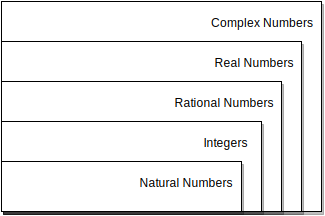
\includegraphics[scale=0.5]{Diagrams/numberClasses}
\par\end{centering}
\caption{\label{fig:numberClassification}The diagram shows the hierarchy of
numbers classified into subsets of the complex numbers.}

\end{figure}


\subsubsection{Composition of Functions}

Let $g$ be a function from the set $A$ to the set $B$and let $f$
be a function from the set $B$ to the set $C$. The \emph{composition
}of the functions $f$ and $g$, denoted for all $a\epsilon A$ by
$f\circ g$. This notation is read ``$f$ of $g$.'' Mathematically,
we then have 
\[
(f\circ g(a))=f(g(a))
\]

Rosen demonstrates this idea with a beautiful depiction of function
composition here given by Figure\vref{fig:functionComposition}.

\begin{figure}
\begin{centering}
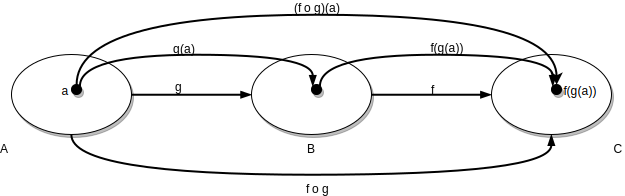
\includegraphics[scale=0.5]{Diagrams/functionComposition}
\par\end{centering}
\caption{\label{fig:functionComposition}The composition of $f$ of $g$. Note
the dependence of the mapping of $f$ by that of $g$. }

\end{figure}


\subsection{The Growth of Functions and Time Complexity}

\subsubsection{Big-O Notation}

Let $f$ and $g$ be functions from the set of integers or the set
of real numbers to the set of real numbers. We say that $f(x)$is
$O(g(x))$ if there are constants $C$and $k$ such that 

\[
|f(x)|\leq C|g(x)|,x>k
\]

The constancs $C$ and $k$ are called witnesses to the relationship
between $f(x)$and $O(g(x))$.

\subsubsection{Big-$\Omega$ and Big-$\Theta$ Notation}

\subsubsection{Time Complexity}

\subsection{Recursion and Induction\label{sec:Induction}}

Inductive mathematical proofs use the true of the basis step and the
truth of a statement implying that if $P(k)$ is true then $P(k+1)$
is also true. When the implication can be proven then we can say for
all integers $n$ the statement $P$ holds true. Rosen provides a
good template for creating proofs using induction. The template follows:
\begin{enumerate}
\item Express the statement that is to be proved in the form \textquotedblleft for
all $n\ge b,P(n)$\textquotedblright , for a fixed integer $b$.
\item Write out the words \textquotedblleft Basis Step.\textquotedblright{}
Then show that $P(b)$ is true, taking care that the correct value
of $b$ is used. This completes the first part of the proof.
\item Write out the words \textquotedblleft Inductive Step.\textquotedblright{}
\item State, and clearly identify, the inductive hypothesis, in the form
\textquotedblleft assume that $P(k)$ is true for an arbitrary fixed
integer $k\ge b$.\textquotedblright{}
\item State what needs to be proved under the assumption that the inductive
hypothesis is true. That is, write out what $P(k+1)$ says.
\item Prove the statement $P(k+1)$ making use the assumption $P(k)$. Be
sure that your proof is valid for all integers $k$ with$k\ge b$,
taking care that the proof works for small values of $k$, including
$k=b$.
\item Clearly identify the conclusion of the inductive step, such as by
saying \textquotedblleft this completes the inductive step.\textquotedblright{} 
\item After completing the basis step and the inductive step, state the
conclusion, namely that by mathematical induction, $P(n)$ is true
for all integers $n$ with $n\ge b$.
\end{enumerate}
\begin{itemize}
\item You can find a good review of \href{http://tutorial.math.lamar.edu/getfile.aspx?file=B,31,N}{algebratic simplification rules}
at the given link.
\end{itemize}

\subsubsection{Strong Induction and Well-Ordering}

To prove that $P(n)$is true for all positive integers $n$, where
$P(n)$ is a propositional function, we complete two steps:
\begin{itemize}
\item \emph{Basis Step}: We verify that the proposition $P(1)$ is true.
\item \emph{Inductive Step: }We show that the conditional statement $[P(1)\land P(2)\land\ldots\land P(k)]\rightarrow P(k+1)$
is true for all positive integers $k.$
\end{itemize}
A good example of the use of strong induction is the proof of the
Fundamental Theorem of Arithmatic. The theorem states all integers
$n$ can be written as the product of two primes.
\begin{thm}
An integer n can be written as the product of two primes.
\end{thm}
The\emph{ well-ordering property} states that every nonempty set of
nonnegative integers has a least element.

\subsection{Modular Arithmetic}

Figure\vref{fig:moduluarArithmatic} gives an overview of basic modular
arithmetic operations. This becomes useful for primality testing. 

\subsubsection{Miller-Rabin Compositeness Test}

//TODO give details on Miller-Rabin

\begin{figure}
\begin{centering}
\begin{tabular}{|c|c|}
\hline 
Arithmetic Property & Equation\tabularnewline
\hline 
\hline 
Modulo Positive Numbers & $a\%b=c$\tabularnewline
\hline 
Modulo Negative Numbers & $c=a-q\cdot b$, where $a<0$, and $-1\leq q\leq\left\lfloor a/b\right\rfloor $\tabularnewline
\hline 
Modular Congruence & $a\%b\equiv b\%c$\tabularnewline
\hline 
Modular Addition & $(a+b)\%c\equiv(a\%c+b\%c)\%c$\tabularnewline
\hline 
Modular Subtraction & $(a-b)\%c\equiv(a\%c-b\%c)\%c$\tabularnewline
\hline 
Modular Multiplication & $(a\cdot b)\%c\equiv(a\%c\cdot b\%c)\%c$\tabularnewline
\hline 
\end{tabular} 
\par\end{centering}
\caption{\label{fig:moduluarArithmatic}This table gives an overview of useful
modular arithmetic equations}
\end{figure}


\subsection{Combinatorics}

You can use counting techniques to answer a variety of questions.
Learning how to account for the time complexity of algorithm will
be very useful in this course.

\subsubsection{The Product Rule}

The product rule is used to count when counting separate tasks. You
should apply this rule when counting nested for loops. Suppose that
a procedure can be broken down into a sequence of two tasks. If there
are$n_{1}$ ways to do the first task and for each of these ways of
doing the first task, there are $n_{2}$ ways to do the second task,
then there are $n_{1}n_{2}$ ways to do the procedure.
\begin{thm}
Suppose that a procedure is carried out by performing the tasks $T_{1},T_{2},\ldots,T_{m}$
in sequence. If each task $T_{i}$ , $i=1,2,\ldots,m$ can be done
in $n_{i}$ ways, regardless of how the previous tasks were done,
then there are $n_{1}\cdot n_{2}\cdot\ldots\cdot n_{m}$ ways to carry
out the procedure.
\end{thm}
\begin{proof}
//TODO Provide an inductive proof of the Product Rule.
\end{proof}
\begin{example}
Assigning tasks to employees. Suppose you hire two employees Ralph
and Loretta. You are tasked with assigning cleaning responsibilities
of $n$ rooms among the two employees. How many ways can you assign
the responsibilities among the employees?
\end{example}
\begin{sol*}
The first employee you select is unrestricted in the number of rooms
to clean. Therefore $n$ rooms may be cleaned by this employee. The
next employee has $n-1$different rooms to clean.
\end{sol*}

\subsubsection{The Sum Rule}

If a task can be done either in one of $n_{1}$ ways or in one of
$n_{2}$ ways, where none of the set of $n_{1}$ ways is the same
as any of the set of $n_{2}$ ways, then there are $n_{1}+n_{2}$
ways to do the task. The key things to look for are a disjunction
of disjoint ways to do a task. Use this rule when counting the number
of steps in a number of sequential for loops. The Sum Rule can be
generalized to $m$ tasks as follows. 
\begin{thm}
Suppose that a task can be done in one of $n_{1}$ ways, in one of
$n_{2}$ ways, $\ldots$ ,or in one of $n_{m}$ ways, where none of
the set of $n_{i}$ ways of doing the task is the same as any of the
set of $n_{j}$ ways, for all pairs $i$ and $j$ with $1\leq i<j\leq m$.
Then the number of ways to do the task is $n_{1}+n_{2}+\ldots+n_{m}$. 
\end{thm}
\begin{proof}
//TODO Provide an inductive proof of the Sum Rule.
\end{proof}

\subsubsection{The Subtraction Rule or The Inclusion Exclusion Principle}

If a task can be done in either $n_{1}$ ways or $n_{2}$ ways, then
the number of ways to do the task is $n_{1}+n_{2}$ minus the number
of ways to do the task that are common to the two different ways.
This rule is often called the principle of inclusion-exclusion especially
when considering the union of sets.

\[
|A_{1}\bigcup A_{2}|=|A_{1}|+|A_{2}|-|A_{1}\bigcap A_{2}|
\]


\subsubsection{The Division Rule}

There are$n/d$ ways to do a task if it can be done using a procedure
that can be carried out in $n$ ways, and for every way $w$, exactly
$d$ of the $n$ ways correspond to way $w$.

\subsubsection{The Pigeonhole Principle (Dirichlet Drawer Principle)}
\begin{thm}
If N objects are placed into k boxes, then there is at least one box
containing at least $\left\lceil N/k\right\rceil $ objects.
\end{thm}
\begin{proof}
We will use a proof by contrapostion. Suppose that none of the boxes
contains more than $\left\lceil N/k\right\rceil -1$ objects. Then,
the total number of objects is at most

\[
k\left(\left\lceil \frac{N}{k}\right\rceil -1\right)<k\left(\left(\frac{N}{k}-1\right)+1\right)=N
\]
This is a contradiction because at most$\left\lceil N/k\right\rceil -1$
were claimed and yet the total is $N.$
\end{proof}
\begin{cor}
A function f from a set with k +1 or more elements to a set with k
elements is not one-to-one.
\end{cor}
\begin{proof}
Suppose that for each element $y$ in the codomain of $f$ we have
a box that contains all elements $x$ of the domain of $f$ such that
$f(x)=y$. Because the domain contains $k+1$ or more elements and
the codomain contains only $k$ elements, the pigeonhole principle
tells us that one of these boxes contains two or more elements $x$
of the domain. This means that $f$ cannot be one-to-one.
\end{proof}

\subsection{Permutations and Combinations}

A \emph{permutation} of the elements of a set is an ordered arrangement
of the elements in the set. A \emph{r-permuation }of a set $S$ is
a permutation of a subset $R\subseteq S$ where $r=|R|$.

An unordered selection of elements of a set is called a \emph{combination.}
An \emph{r-combination} of elements of a set is an unordered selection
of \emph{r} elements from the set.

A combinatorial proof of an identity is a proof that uses counting
arguments to prove that both sides of the identity count the same
objects but in different ways or a proof that is based on showing
that there is a bijection between the sets of objects counted by the
two sides of the identity. These two types of proofs are called double
counting proofs and bijective proofs, respectively.

\begin{figure}
\begin{centering}
\begin{tabular}{|c|c|c|}
\hline 
Type & Repetition Allowed? & Formula\tabularnewline
\hline 
\hline 
r-permutations & No & $\frac{n!}{(n-r)!}$\tabularnewline
\hline 
r-combinations & No & $\frac{n!}{r!(n-r)!}$\tabularnewline
\hline 
r-permutations & Yes & $n^{r}$\tabularnewline
\hline 
r-combinations & Yes & $\frac{(n+r-1)!}{r!(n-1)!}$\tabularnewline
\hline 
\end{tabular}
\par\end{centering}
\caption{\label{fig:permCombFormulas}Formulas for calculating permutations
and combinations.}

\end{figure}


\subsection{Probability and Statistics\label{sec:Probability-and-Odds}}

First we introduce some nomenclature for this domain of study. 
\begin{itemize}
\item An \emph{experiment} is a procedure that yields one of a given set
of possible outcomes.
\item The\emph{ sample space} of the experiment is the set of possible outcomes.
\item An \emph{event} is a subset of the sample space.
\end{itemize}
Laplace defines the probability of an event as given a set S, a finite
nonempty sample space, of equally likely outcomes, and $E$ is an
event, that is, $E\subseteq S$, then the probability of $E$ is $p(E)=\frac{|E|}{|S|}.$
The probability of the complement of an event is $\bar{E}=S-E$, and
the complementary event is given by $p(\bar{E})=1-p(E)$.

We can find the probability of the union of events by adding their
probabilities and subtracting the intersection of the events. 
\[
p(E_{1}\bigcup E_{2)}=p(E_{1})+p(E_{2})-p(E_{1}\bigcap E_{2}).
\]


\subsubsection{Nonuniform Probability}

In the previous section we operated under the conditions of equal
probability for each event in the sample space. However, many questions
may be posed where this is not the case. To account for nonuniform
probability of events we must introduce two constraints on the members
of the sample pace $S$.
\begin{enumerate}
\item $0\leq p(s)\leq1$, The probability of each element in the samples
space must be between 0 and 1.
\item $\sum_{s\epsilon S}p(s)=1$, The sum of the probabilities of each
element of $S$ must be 1.
\end{enumerate}

\subsubsection{Conditional Probability}

Let $E$ and $F$ be events with $p(F)>0$. The conditional probability
of $E$ given $F$, denoted by $p(E|F).$

\[
p(E|F)=\frac{p(E\bigcap F)}{p(F)}
\]

\emph{Independent events} are events that do not affect each other.
When two events are independent, the occurrence of one of the events
gives no information about the probability that the other event occurs.
Mathematically, if $p(E)=p(E|F)$ then the events $E$ and $F$ are
said to be independent.

Pairwise independence is defined as follows: The events $E_{1},E_{2},\ldots,E_{n}$
are \emph{pairwise independent }if and only if $p(E_{i}\bigcap E_{j})=p(E_{i})p(E_{j})$
for all integers $i$ and $j$ with $1\leq i<j\leq n$. Events are
said to be \emph{mutually independent }if the following is true
\[
(E_{i_{1}}\bigcap E_{i_{2}}\bigcap\ldots\bigcap E_{i_{m}})=p(E_{i_{1}})p(E_{i_{2}})\ldots p(E_{i_{m}})
\]
when for $i_{j}$, $1<j\leq m$ and $1\leq i_{1}<i_{2}<\ldots<i_{m}\leq n$.
It should be noted that all mutually independent events are also pairwise
independent, but not all pairwise independent events are mutually
independent.

\subsubsection{Bernoulli Trials}

An experiment that only has two possible outcomes is called a \emph{Bernoulli
trial. }Bernoulli trials consist of independent events. Examples of
such experiments include flipping a coin and generating bits at random.
\begin{thm}
The probability of exactly k successes in n independent Bernoulli
trials, with probability of success p and probability of failure q
= 1\textminus p, is

\[
C(n,k)p^{k}q^{n-k}
\]
\end{thm}
\begin{proof}
When $n$ Bernoulli trials are carried out, the outcome is an n-tuple
$(t_{1},t_{2},\ldots,t_{n)}$. Wherefore $t_{i}$, from $1\leq i\leq n$
each is denoted $S$ in a successful trial and $F$ in a failed trial.
Because the $n$ trials are independent the probability of $k$ success
and $n-k$ failures is $p^{k}q^{n-k}$. Further, there are $C(n,k)$tuples
in which there are $k$ successes, and so the probability is $C(n,k)p^{k}q^{n-k}$.
\end{proof}

\subsubsection{Random Variables}

(Possibly the most poorly named concept in mathematics) A random variable
is a \emph{function} from the sample space of an experiment to the
set of real numbers. That is, a random variable assigns a real number
$r$ to each possible outcome.

The distribution of a random variable $X$ on a sample space $S$
is the set of pairs $(r,p(X=r))$ for all $r$ $\epsilon$ $X(S)$,
where $p(X=r)$ is the probability that $X$ takes the value $r$.
(The set of pairs in this distribution is determined by the probabilities
$p(X=r)$ for $r\in X(S).)$

\subsubsection{Probablistic Algorithms}

Probabilitic algorithms are algorithims that make a random choice
at some step during computation. This strikes a contrast with determinitic
algorithms which proceed step by step with each successive step defined
explicitly by the source code. For a sufficiently large number of
computations the chances that a probabilitic algorithm will yield
a correct answer to a decision problem increases dramatically. Probablistic
algorithms are traditionally classified as Monte Carlo type or Las
Vegas type algorithms.

\subsubsection{Monte Carlo Algorithms}

For a sufficiently large number of computations the chances that a
Monte Carlo algorithm will yield a correct answer to a decision problem
increases dramatically. However, a chance remains that an incorrect
answer will be given. During the computation of a Monte Carlo algorithm
a series of tests are run that return a either true, false, or unknown.
After a sufficient number of iterations are run if any of the tests
returned a true response then the algorithm will respond in the affirmative.
However if every test responded with an unkown status then the algorithm
will respond false.

\subsubsection{Las Vegas Algorithms}

\subsubsection{The Probabilistic Method}

The Pobablistic Method states that if the probability that an element
chosen at random from a $S$ does not have a particular property is
less than 1 (the is some uncertantity), then there exists an element
in S with this property.

\subsubsection{Expected Value and Variance}

The \emph{expected value} of a random varariable (chance function)
is the sum over all the elements of the sample space of the probability
of the element times the value of the random variable at this element
(i.e. it is the weighted average of the random variable). The expected
value gives us a targeted value at which the distribution of the random
variable's probability curve. Formally, the expected value, also called
the expectation or mean, of the random value $X$on the sample space
$S$ is equal to:
\[
E(X)=\sum_{s\epsilon S}p(s)X(s)
\]
 The \emph{deviation }of X at $s\epsilon S$ is $X(s)-E(x)$, the
difference between the value of $X$and the mean of $X.$

In cases where computing the expected value directly is infeasible
because the size of the sample space is too large we can use the following
theorem to compute the expected value by grouping outcomes by their
value and multiplying them times their respective probabilities.
\begin{thm}
If X is a random variable and p(X=r) is the probability that X will
be r, so that the $\sum_{s\epsilon S,X(s)=r}p(s)$, then:

\[
E(X)=\sum_{r\epsilon X(S)}p(X=r)r
\]
\end{thm}
\begin{proof}
Suppose that $X$ is a random variable with range $X(S)$, and let
$p(X=r)$ be the probability that the random variable $X$ takes the
value $r$. Consequently, $p(X=r)$ is the sum of the probabilities
of the outcomes $s$ such that $X(s)=r$. It follows that

\[
E(X)=\sum_{r\epsilon X(S)}p(X=r)r
\]
\end{proof}
\begin{thm}
The Linearity of Expectations states that if for a random variable
$X_{i}$, $i=1,2,\ldots n$, are random variables on the sample space
$S$. and if $a$and $b$ are real numbers then
\end{thm}
\begin{enumerate}
\item 
\[
E(X_{1}+X_{2}+\ldots+X_{3})=E(X_{1})+E(X_{2})+\ldots+E(X_{n})
\]
\item 
\[
E(aX+b)=aE(X)+b
\]
\end{enumerate}
Variance tells us the spread of the values of the random variable.
Let X be a random variable on a sample space S. The variance of X,
denoted by V(X), is:

\[
V(X)=\sum_{s\epsilon S}(X(s)-E(X))^{2}p(s)
\]


\subsubsection{Chebyshev's Inequality}

Chebyshev's inequality helps us answer how likely it is that the outcome
of a random variable will be significanyly more than its expected
value. Chebychev provides an upper bound on the probability that the
value of a random variable differs from the expected value of the
random variable by more than a specified amount.
\begin{thm}
Let X be a random variable on a sample space S with probability function
p. If r is a positive real number, then

\[
p(|X(s)-E(X)|\ge r)\le V(X)/r^{2}.
\]
\end{thm}

\section{Linear Algebra\label{sec:Linear-Programming}}

\subsection{Linear Equations in Linear Algebra}

\subsection{Matrix Algebra}

\subsection{Determinants}

\subsection{Vector Spaces}

\subsection{Eigenvalues and Eigenvectors}

\subsection{Orthogonality and Least Squares}

\subsection{Symmetric Matrices and Quadratic Forms}

\subsection{Geometry of Vector Spaces}

\subsection{Basic Properties of Linear Programs}

\subsection{The Simplex Method}

\subsection{Duality and the Complementary}

\subsection{Interior Point Methods}

\part{Computability}

\section{Deterministic Finite Automata\label{sec:deterministicFiniteAutomata}}

Finite automata are a systems of information represented by states,
transitions, and inputs. Information about the computation is derived
from the state in which the automata exists and no previous information
can be remembered by the finite automata. The limits to which the
finite automata can model information are expressed by the number
of states.

\subsection{Notation of DFA's\label{subsec:Notation-of-DFA's}}

Traditionally, finite automata\index{automata} are expressed by a
tuple which express its behavior. The tuple, for example $L=(Q,\Sigma,\delta,q_{0},F)$.
\begin{itemize}
\item The contains information on the states expressed by the set Q.
\item The input alphabet\index{alphabet} expressed by the set $\Sigma$.
\item The transitions\index{transitions} expressed by the function $\delta$.
\item The starting state given by $q_{0}$.
\item The set of final states given by $F$. 
\end{itemize}
An example of a finite automata can be seen in Figure\ref{fig:productDFA}.
Strings are typically represented by variables of lowercase letters
at the end of the alphabet \emph{(w, x, y, and z).} Whereas, characters
are represented variables of lowercase letters at the beginning of
the English alphabet \emph{(a, b, and c).} 

$\Sigma^{*}$ represents the set of all strings over the alphabet
$\Sigma$ including the empty string, $\varepsilon$. The super-script
star symbol is referred to as the Kleene star\index{Kleene star}.
The empty string denotes a string of length 0, a string of no characters
``''.

Length, sometimes called cardinality, is often expressed by vertical
bars surrounding the string in question, such as $|w|$.

A transition function $\delta$ takes two parameters, a state and
an input symbol, and returns the next state to which the automaton
should transition on input of the symbol ( i. e. $\delta(q,$a)). 

\subsection{Computation of DFA's\label{subsec:Computation-of-DFA's}}

Given a finite automata, computation can be carried out on an input
string by processing each character of the input one-by-one and following
the transitions based on the input character. Upon encountering the
last character in the input string computation stops. The string is
either accepted or rejected and based on whether the state is a final
state (accepting state) or a nonaccepting state. 

Accepted strings are said to be in the language of the automaton,
and rejected strings are not in the language. Given an automaton $A$
the language of $A$ is denoted $L(A)$. A language is a subset of
$\Sigma^{*}$.

\subsection{Regular Languages\label{subsec:Regular-Languages}}

\emph{A language is a regular language\index{regular language} if
it is accepted by some \index{deterministic finite automata (DFA}deterministic
finite automata (DFA)}. A caveat here is that the DFA must accept
only those strings in the language it models and no others.

Nonregular languages are those that cannot be modeled by a DFA. Examples
of nonregular languages are those that require automata to count beyond
a finite number of states. 

The classical example is the language L = \{$0^{n}1$$^{n}$ | $n\geq1$\}.
DFA's cannot check for the same number of symbols in a string or balanced
parenthesis. This job falls to context free grammars (CFG) outlined
in section \vref{sec:contextFreeGrammars}.

\section{Nondeterministic Finite Automata\label{sec:Nondeterministic-Finite-Automata}}

A \index{nondeterministic finite automaton (NFA)}nondeterministic
finite automaton (NFA) differs from its deterministic counterpart
in that it may be in many states at once. Transitions on an input
symbol may proceed to any number states. This idea is demonstrated
in Figure\vref{fig:nfaExample}. NFA's are equivalent to DFA's and
such anything that can be modeled with a NFA can be modeled with a
DFA. Thus, the class of languages modeled by NFA's is the regular
languages.

\begin{figure}
\begin{centering}
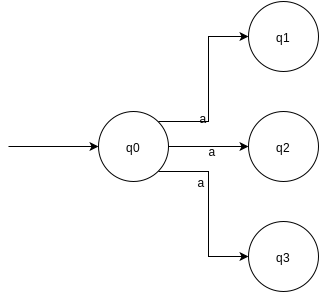
\includegraphics[scale=0.5]{Diagrams/nfaExample}
\par\end{centering}
\caption{\label{fig:nfaExample}The NFA depicted in the diagram shows that
on input symbol $a$the automaton transitions to the state $q_{1},q_{2}$
and $q_{3}$ at the same time. }

\end{figure}


\subsection{Proof of Equivalence of NFA's and DFA's\label{subsec:Proof-of-Equivalence}}

The proof of equivalence between DFA's and NFA's is often called the
Subset Construction. 

In the following proof given a NFA the states $Q_{N}$, inputs $\Sigma$,
transition function $\delta_{N}$, start state q, and final states
$F$. The set of states of the constructed DFA $Q_{D}$ = 2$^{Q_{N}}$,
that is the power set of the set of states of the NFA. A power set
of a set is defined as the set of all possible subsets of a given
set. The inputs to the DFA will be the same as the inputs of the NFA,
$\Sigma$. The start state of the DFA is the set containing the start
state, $q_{0}$ of the NFA. The DFA states are named such that they
enumerate the powerset's subsets with labels that correspond to the
states of the NFA. The transition function for the DFA, $\delta_{D}$
is defined by $\delta_{D}(\{q_{1,}q_{2},\ldots q_{k}\},a)$ is the
union over all i, for$i=1\ldots k$ of the NFA's transition function
$\delta_{N}(q_{i},a)$. 
\begin{thm}
All NFA's have an equivalent DFA representation. Formally, $\delta_{N}(q_{0},w)=\delta_{D}(\left\{ q_{0}\right\} ,w)$. 
\end{thm}
\begin{proof}
The proof is an induction on the string $w$. For the basis step we
take $w=\epsilon$ : $\delta_{N}(q_{0},\epsilon)=\delta_{D}(\left\{ q_{0}\right\} ,\epsilon)=\{q_{0}\}$
. This is true by the basis rule for extending the delta function
for NFA's and DFA's. We assume that the inductive hypothesis holds
from strings shorter than $w$. Let $w=xa$. The inductive hypothesis
holds from the string $x$. Let $\delta_{N}(q_{0},x)=\delta_{D}(\{q_{0}\},x)=S.$
$S$ represents a label for a set of states of the NFA. Let $T$ be
the union over all states $p$ in $S$ of $\delta_{N}(p,a).$ Then
$\delta_{N}(q_{0},w)=\delta_{D}(\{q_{0}\},w)=T$ by the rule for extending
delta functions of NFA's and DFA's. Thus, DFA's and NFA's are equivalent.
\end{proof}

\subsection{Conversion from NFA to DFA\label{subsec:Conversion-from-NFA}}

An example of a transition function on a chess board shown in Figure\vref{fig:chessBoard}
is given by the NFA's transition table in Figure\vref{fig:convertNFA2DFA}.
An equivalent DFA transition table is given by the adjoining table
in the diagram. A lazy conversion technique can be carried out to
only include the state sets in the DFA only when necessary. An automaton
modeling the NFA representation of the chess board is depicted in
Figure\vref{fig:chessNFA2}. A corresponding DFA automaton representation
is depicted in Figure

\begin{figure}
\begin{centering}
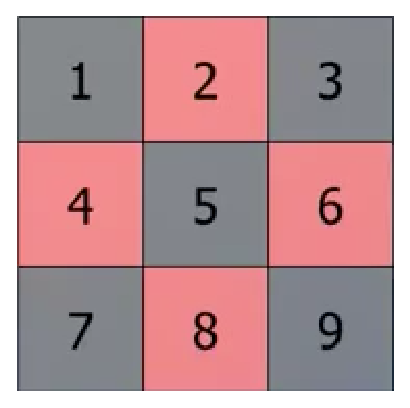
\includegraphics[scale=0.5]{Diagrams/chessBoard}
\par\end{centering}
\caption{\label{fig:chessBoard} A traditional chess board enumerating the
black and red squares with odd and even numbers, respectively. In
this board a transition onto state $9$ constitutes an accepting state.}

\end{figure}

\begin{figure}
\begin{centering}
\begin{tabular}{|c|c|c|}
\hline 
NFA & r & b\tabularnewline
\hline 
\hline 
1 & 2,4 & 5\tabularnewline
\hline 
2 & 4,6 & 1,3,5\tabularnewline
\hline 
3 & 2,6 & 5\tabularnewline
\hline 
4 & 2,8 & 1,5,7\tabularnewline
\hline 
5 & 2,4,6,8 & 1,3,7,9\tabularnewline
\hline 
6 & 2,8 & 3,5,9\tabularnewline
\hline 
7 & 4,8 & 5\tabularnewline
\hline 
8 & 4,6 & 5,7,9\tabularnewline
\hline 
{*}9 & 6,8 & 5\tabularnewline
\hline 
\end{tabular} %
\begin{tabular}{|c|c|c|}
\hline 
DFA & r & b\tabularnewline
\hline 
\hline 
$\left\{ 1\right\} $ & $\left\{ 2,4\right\} $ & $\left\{ 5\right\} $\tabularnewline
\hline 
$\left\{ 2,4\right\} $ & $\left\{ 2,4,6,8\right\} $ & $\left\{ 1,3,5,7\right\} $\tabularnewline
\hline 
$\left\{ 5\right\} $ & $\left\{ 2,4,6,8\right\} $ & $\left\{ 1,3,7,9\right\} $\tabularnewline
\hline 
$\left\{ 2,4,6,8\right\} $ & $\left\{ 2,4,6,8\right\} $ & $\left\{ 1,3,5,7,9\right\} $\tabularnewline
\hline 
$\left\{ 1,3,5,7\right\} $ & $\left\{ 2,4,6,8\right\} $ & $\left\{ 1,3,5,7,9\right\} $\tabularnewline
\hline 
{*}$\left\{ 1,3,7,9\right\} $ & $\left\{ 2,4,6,8\right\} $ & $\left\{ 5\right\} $\tabularnewline
\hline 
{*}$\left\{ 1,3,5,7,9\right\} $ & $\left\{ 2,4,6,8\right\} $ & $\left\{ 1,3,5,7,9\right\} $\tabularnewline
\hline 
\end{tabular}
\par\end{centering}
\caption{\label{fig:convertNFA2DFA} In the transition table for either the
NFA or DFA. Odd numbered states can be viewed as the black squares
of a chess board while even numbered states are the red squares. Note
that the list of states in the NFA transitions expresses the fact
that the NFA transitions to the enumerated states simultaneously,
while the DFA bracketed states express the label of the single state
to which the DFA transitions on the input symbol. In the DFA table
the state set label $\left\{ 2,4\right\} $ is assigned the state
$\left\{ 2,4,6,8\right\} $ on input r because it represents the union
of the transitions of the states to which the NFA will transition
to on input r from either state 2 or 4. This logic applies for all
other states set given in the DFA table as well. Star symbols in either
table indicate a final state.}
\end{figure}

\begin{figure}
\begin{centering}
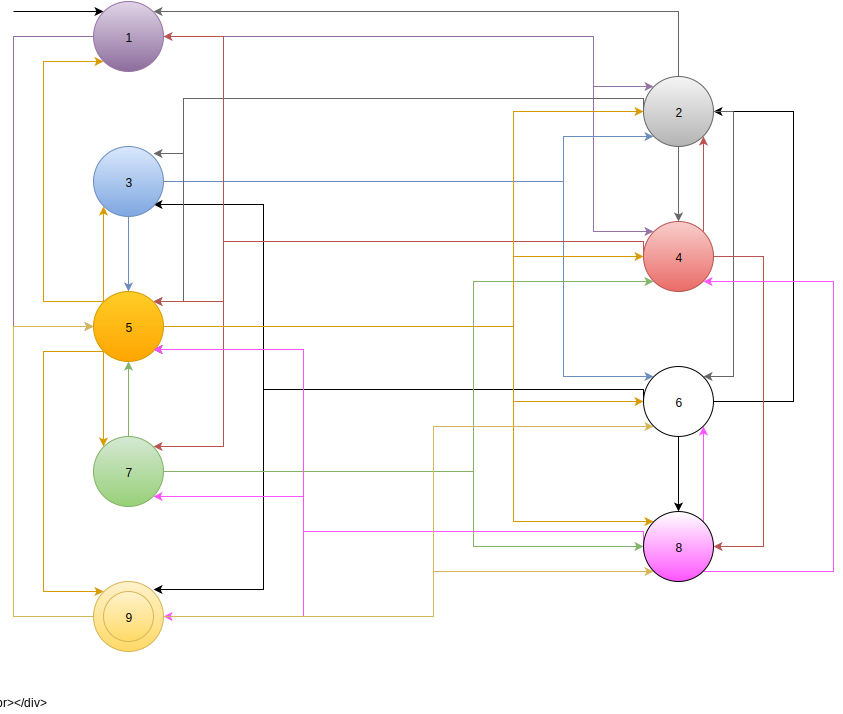
\includegraphics[scale=0.5]{Diagrams/chessNFA2}
\par\end{centering}
\caption{\label{fig:chessNFA2} The chess NFA automaton. Transitions from odd
numbers to even numbers occur on the input symbol $r$. Transitions
from even numbers to odd numbers occur on input symbol $b$. Transition
labels have been omitted for the sake of clarity.}

\end{figure}

\begin{figure}
\begin{centering}
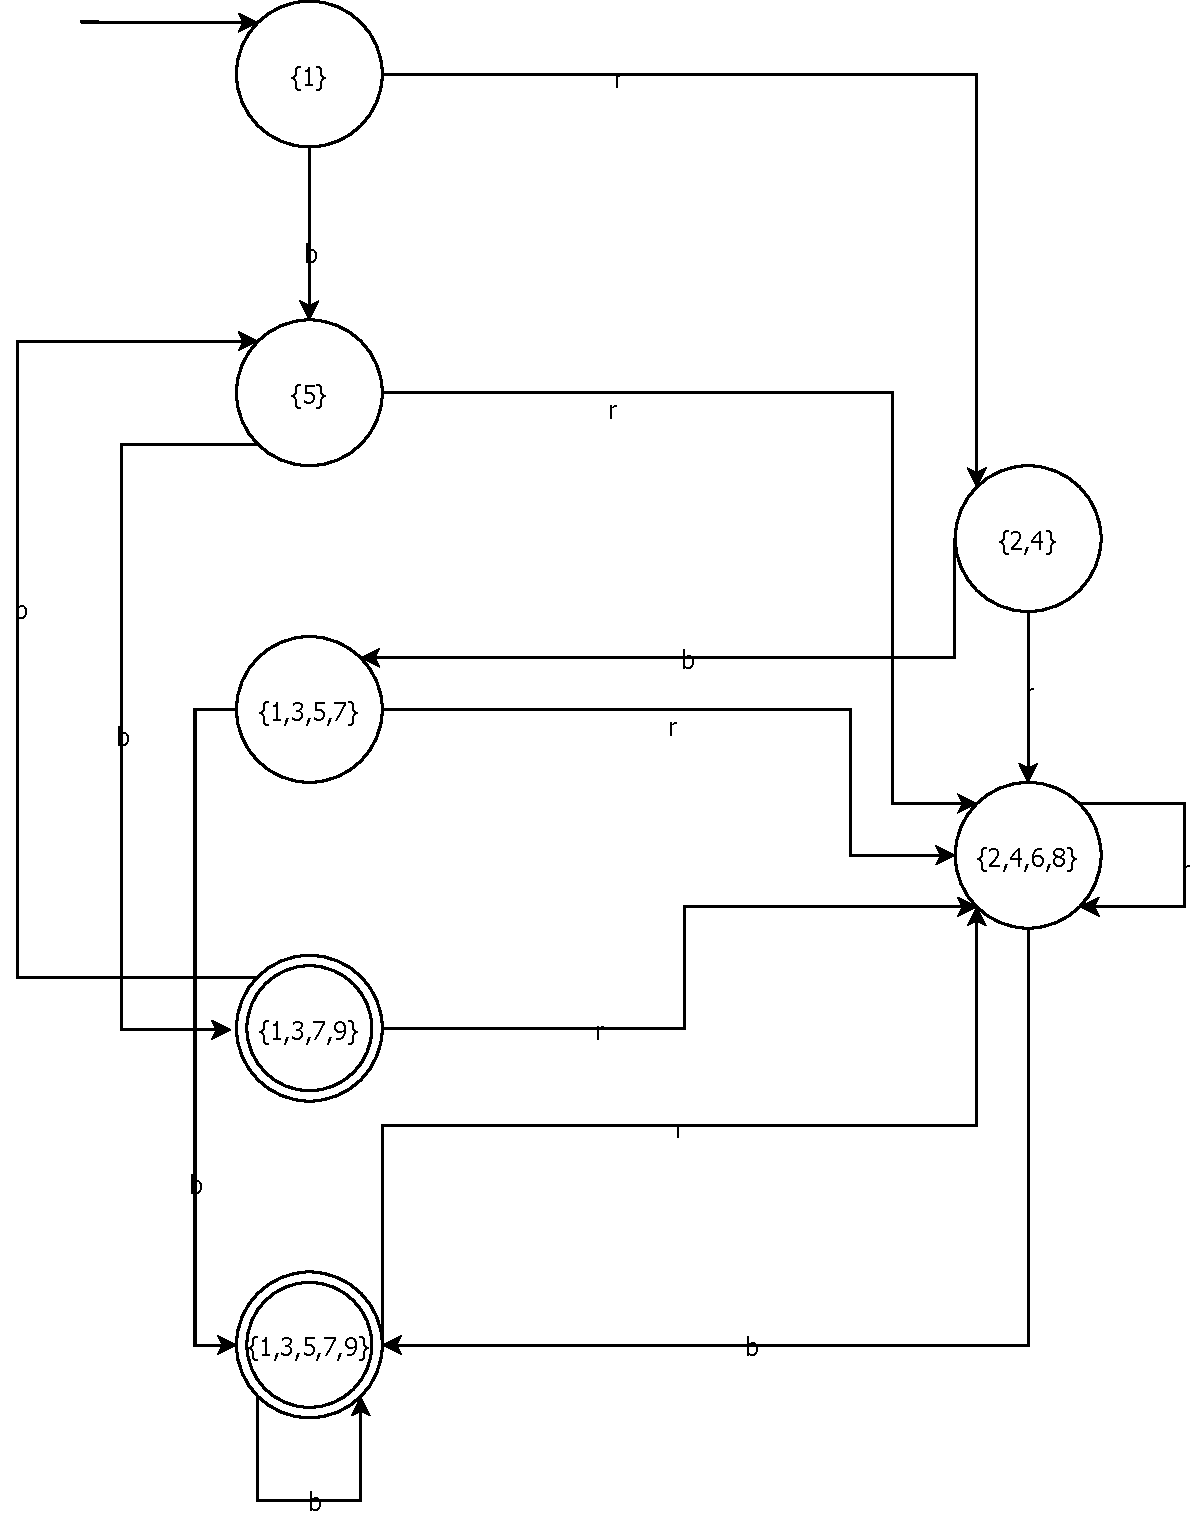
\includegraphics[scale=0.5]{Diagrams/chessDFA}
\par\end{centering}
\caption{\label{fig:chessDFA} The chess DFA automaton.}

\end{figure}


\section{$\epsilon-$NFA's\label{sec:epsilonNFA's}}

NFA's that allow for epsilon transitions are called epsilon NFA. Epsilon
transitions allow for an automaton to transition between states without
regard to the input string. Effectively, it allows for the computation
to skip forward in the automaton without processing input. An example
of an epsilon NFA is depicted in Figure\vref{fig:epsilonNFA}.

\begin{figure}
\begin{centering}
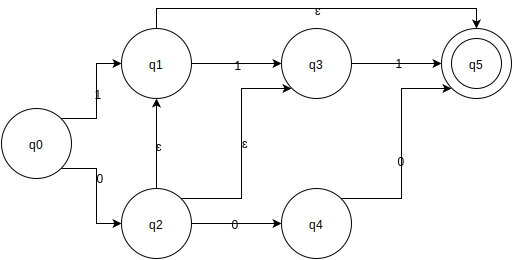
\includegraphics[scale=0.5]{Diagrams/epsilonNFA}
\par\end{centering}
\caption{\label{fig:epsilonNFA} Epsilon transitions are marked with a $\epsilon$symbol.
Upon transitioning to state $q_{2}$ the automaton spontaneously and
in parallel transitions to states $q_{1}$, $q_{3}$ and $q_{5}$. }
\end{figure}


\subsection{Closure of States\label{subsec:Closure-of-States}}

The closure of states is defined as the set of states reachable from
state in question. The function is traditionally denoted $CL(q).$
The closure of state $q2$ in Figure \vref{fig:epsilonNFA} is $\left\{ q2,q1,q3,q5\right\} $.

\section{Regular Expressions\label{sec:Regular-Expressions}}

Regular expressions use three operations: union, concatenation, and
Kleene star. Concatenation on languages $L$ and $M$is denoted $LM.$
$LM$ is defined as $wx$ where $w\varepsilon L$ and $x\varepsilon M$.
Kleene star ($^{*})$ is the set of strings formed by concatenating
0 or more strings of $L$ in any order. The Kleene star of $L$ is
then $L^{*}=\left\{ \epsilon\right\} \cup L\cup LL\ldots$ 

\subsection{Precedence of Operators on Regular Expressions\label{subsec:Precedence-of-Operators}}
\begin{enumerate}
\item Parenthesis
\item Kleene star
\item Concatenation
\item Union
\end{enumerate}

\subsection{Algebraic Laws and Identities of Regular Expressions\label{subsec:algebraicLawsAndIdentitesRegularLanguages}}

Union is commutative and associative. Concatenation is associative
however is not commutative.$\emptyset$ is the identity for union.$\epsilon$is
the identity for concatenation. $\emptyset$ is the annihilator for
concatenation.

\section{Properties of Language Classes\label{sec:propertiesOfLanguages}}

A language class is a set of languages, and language classes have
two important properties.
\begin{itemize}
\item Decision properties\index{decision properties} - algorithms that
when applied to a language determine whether a certain property holds
(e.g. is a language empty).
\item Closure properties\index{closure properties} - describes the operations
in which when applied to a language class produce another language
in the same language class (e.g. union)
\end{itemize}

\subsection{Decision Properties of Regular Languages\label{subsec:DecisionPropertiesOfRegularLanguages}}

\subsubsection{The Membership Test for Regular Languages\label{subsec:membershipTestForRegularLanguages} }

The classic decision property for languages is the Membership Test.
That is, is a given string w in the language. The algorithm to determine
this is simply to simulate the string on the DFA of the language.
If the simulation of w on the DFA ends in an accepting state, then
the string is in the language, otherwise the string has ended in a
non-accepting state of the DFA and it is thus not in the language. 

\subsubsection{The Emptiness Test for Regular Languages\label{subsec:emptinessTestForRegularLanguages}}

Another example of decision properties is the Emptiness Problem. That
is given a regular language, does it contain any strings at all? To
determine whether the language has any strings first obtain the DFA-representation
of the language and then compute the reachable states from the start
state. A good way of doing this is Breadth-First Search on the graph
of the DFA. If a accepting state is reachable from the start state
then we know that at least one string is in the language.

\subsubsection{The Equivalence Test for Regular Languages\label{subsec:equivalenceTestForRegularLanguages}}

Another example of decision properties is testing whether two languages,
L and M, are equivalent. Their DFA's are specified as follows: $L=(Q,\Sigma,\delta_{L},A,F_{L})$
and $M=(R,\Sigma,\delta_{M},C,F_{M})$ where $Q=\{A,B\}$, $R=\left\{ C,D\right\} $,
and $\Sigma=\{0,1\}$. The transition function on each DFA, L and
M can be seen in Figure\vref{fig:productDFA}. To test equivalence
one may form a product on the states of each DFA such that for each
respective state in Q and R the product DFA's state set is $Q\times R$
has a corresponding state. The start state for the product DFA would
then be the pair $\left[q_{0},r_{0}\right]$ . The transition function
would then be formed as follows: $\delta(\left[q,r\right],1)=\left[\delta_{L}(q,1),\delta_{M}(r,1)\right]$.
The product DFA N pictured in Figure\vref{fig:productDFA} is assigned
final states such that either the one of the state pair's respective
DFA enters a final state, but not both. For example, the state B is
a final state in the DFA L, and the state C is a final state in the
DFA M. The state pair (B,D) is then marked final in the DFA N instead
of (B,C) because the state D is not a final state in the DFA M. Similarly,
the state pair (A,C) is marked a final state in the DFA N because
C in final state the DFA M, but A is not a final state in the DFA
L. This feature of only one state being accepting is used a differentiating
characteristic to determine whether the languages of the DFA's L and
M are equivalent. The languages L and M are equivalent if and only
if the language of N is empty. This means that N models the feature
that neither L accepts when M does not, nor does M accept when L does
not. It is clear from the that the empty string $\epsilon$ is accepted
by M and not by L and is so modeled by the pair (A,C) in N. N accepts
the empty string and therefore, L and M are not equivalent languages.

\begin{figure}
\begin{centering}
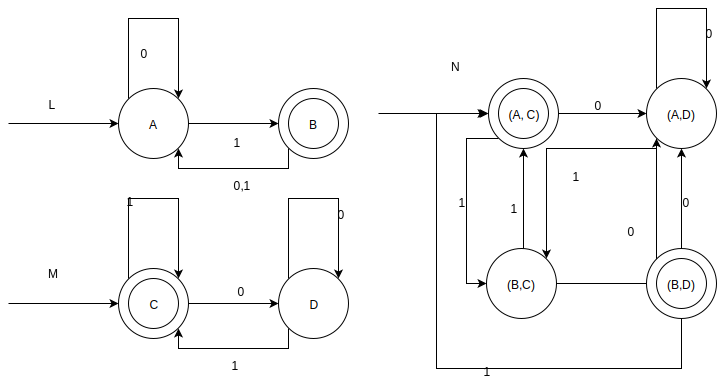
\includegraphics[scale=0.5]{Diagrams/productDFA}
\par\end{centering}
\caption{\label{fig:productDFA}The transition function formed on newly formed
state set of $Q\times R$ corresponds to the transitions of L and
M. }

\end{figure}


\subsubsection{The Infiniteness Test for Regular Languages\label{subsec:infinitenessTestRegularLanguages}}

A final example of decision problems fro regular languages in the
Infiniteness Problem. The problem asks, is the given regular language
composed of an infinite number of strings? We can determine if a given
language is infinite by examining the DFA-representation of the language.
If the DFA has n states, and the given language has a string of n
or more in length, then the language is infinite. Otherwise, the language
must be finite. (If a language has a string of length n or more, then
surely the DFA contains a cycle that yielded such a string). The proof
of this idea follows: If there is a n-state DFA that accepts a string
w of length n or more, then there must be a state that appears twice
on the path traced out by the simulation of w on the DFA from the
start state to the final state. This is because for all strings w
of length n a DFA must traverse n+1 states. A diagram of the automaton
demonstrating this principle can be seen in Figure \vref{fig:pumpingLemma}.

\noindent 
\begin{figure}
\centering{}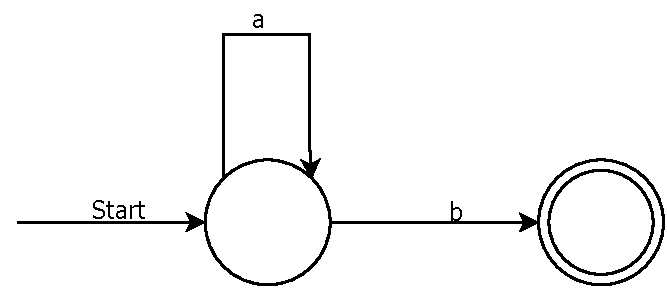
\includegraphics[scale=0.5]{Diagrams/pumpingLemma}\caption{\label{fig:pumpingLemma}In the automaton pictured above a string
w is formed by the the substrings x, y, and z. The substring x is
the substring that takes us to the first cycle in the automaton. The
cycle occurs at state q. The edge labeled y represents the edge which
returns the string w to state q for the first time. Because the substring
y is locked within the string w, that is its prefix is the substring
x and its postfix is the substring z, it cannot be the empty string.
However, the substrings x or z may be the empty string. Then $xy^{i}z$
for all $i\geq0$ is in the language, and therefore an infinite number
of strings exist in the language.}
\end{figure}

\begin{thm}
If there is a string w=xyz of length $\geq n$ in L, then there is
a string of length $\left[n,2n-1\right]$ . 
\end{thm}
\begin{proof}
Because y is the first cycle on the path to the accepting state, the
length $|xy|\leq n$, and more specifically, $1\leq|y|\leq n$ ( x
and z may be empty strings). Some state along the path xy surely must
repeat. If w is the shortest possible string of length n, then it
cannot be longer than 2n. However, suppose it was. The string xz is
another accepted string in the language. We know that xz = w - y,
and the length of $y\leq n$, so the length of $xz\geq n$. Which
means that $|xz|\leq|w|$, and yet at least n in length which is accepted,
but we assumed that the were no strings that were shorter than w and
of length at least n. Thus, if the string w were of length $\geqq2n$
, there is a shorter string of length $\left[n,2n-1\right]$ formed
by removing the substrings represented by y which are $\left[1,n\right]$
. 
\end{proof}

\subsection{Closure Properties of Regular Languages\label{subsec:closurePropertiesOfRegularLanguages}}

\subsubsection{Union for Regular Languages\label{subsec:UnionForRegularLanguages}}

If $L$ and $M$ are regular languages, then $L\cup M$ is also a
regular language. The proof of this statement is as follows: Let the
languages $L$ and $M$ be the languages of the regular expressions
$R$ and $S$ respectively, then $R+S$ is a regular expression whose
language is the $L\cup M$. 

\subsubsection{Intersection for Regular Languages\label{subsec:IntersectionForRegularLanguages}}

If $L$ and $M$ are regular languages, then $L\cap M$ is also a
regular language. The proof of this statement is as follows: Let $I$
and $J$ be the DFA's for the regular languages $L$ and $M$, respectively.
Form the product DFA $K$ of $I$ and \textbf{$J$ }and mark the final
states of $K$ as the states in which both $I$ and $J$ are in final
states. The DFA $K$ is now a regular language representing $L\cap M$.
This idea is demonstrated in Figure\vref{fig:intersectionDFA}.

\begin{figure}
\begin{centering}
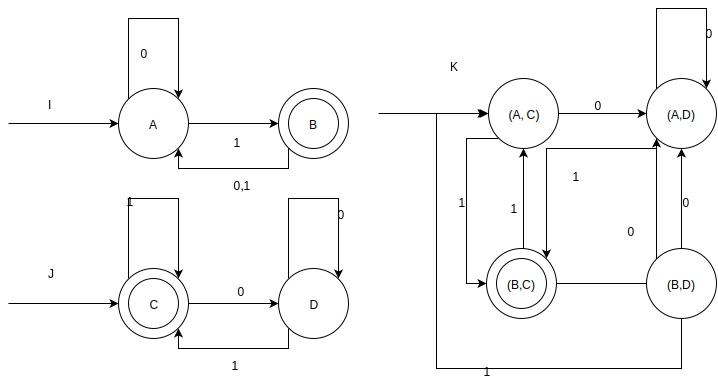
\includegraphics[scale=0.5]{Diagrams/intersectionDFA}
\par\end{centering}
\caption{\label{fig:intersectionDFA}The product DFA $K$ represents the intersection
of $L$ and $M$ and its final state is the state pair for which a
final state exists for both $I$ and $J$. }

\end{figure}


\subsubsection{Difference for Regular Languages\label{subsec:DifferenceForRegularLanguages}}

If $L$ and $M$ are regular languages, then $L-M$ is also a regular
language. $L-M$ represents the strings that are in $L$ but not in
$M$. The proof of this statement is as follows: Let $I$ and $J$
be the DFA's for the regular languages $L$ and $M$, respectively.
Form the product DFA $K$ of $I$ and \textbf{$J$ }and mark the final
states of $K$ as the states in which $I$ is in a final state and
$J$ is not in a final state. The DFA $K$ now represents $L-M$.

\subsubsection{Concatenation for Regular Languages\label{subsec:ConcatenationForRegularLanguages}}

If $L$ and $M$ are regular languages, then $LM$ is also a regular
language. The proof of this statement is as follows: Let the languages
$L$ and $M$ be the languages of the regular expressions $R$ and
$S$ respectively, then $RS$ is a regular expression whose language
is the $LM$.

\subsubsection{Kleene Closure for Regular Languages\label{subsec:KleeneClosureForRegularLanguages}}

$R^{*}$ is a regular expression whose language is $L^{*}$.

\subsubsection{Complement for Regular Languages\label{subsec:ComplementForRegularLanguages}}

The complement of a language $L$ with respect to an alphabet $\Sigma$
such that $\Sigma^{*}$contains $L$ is the difference of $\Sigma^{*}$
and the language $L$. Since $\Sigma^{*}$ is surely a regular language,
and regular languages are closed under difference as we have seen
previously, then the complement $\Sigma^{*}-L$ is also regular.

\section{Conversion of Language Representations\label{subsec:conversionOfLanguageRepresentations}}

A cycle is formed on the way in which we can represent languages.
There exists algorithms to convert from one representation to the
next along the cycle depicted in Figure\vref{fig:representationCycle}.
As such, given a regular expression one may convert it to a DFA.

\begin{figure}
\begin{centering}
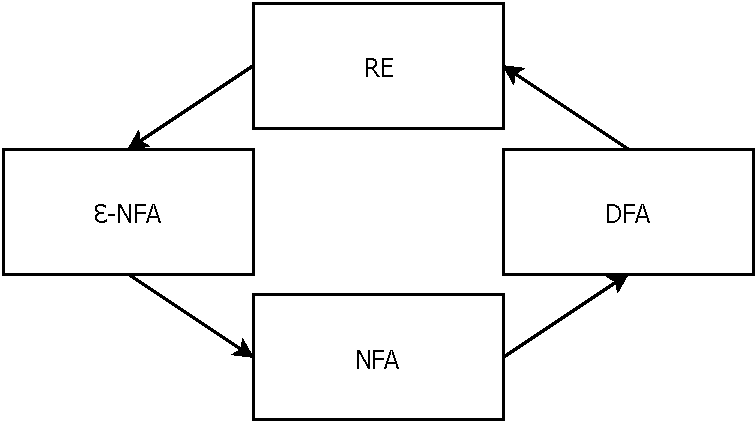
\includegraphics[scale=0.5]{Diagrams/representationCycle}
\par\end{centering}
\caption{\label{fig:representationCycle} This diagram describes the conversion
cycle of representations such that from a regular expression it is
possible to obtain a DFA. }
\end{figure}


\section{DFA Minimization\label{sec:DFA-Minimization}}

Minimizing a DFA can be carried out in a naive way by enumerating
all smaller DFA's for any given DFA and checking for equivalence.
However, this is terribly inefficient and a smarter algorithm can
be used to generate a equivalent DFA much faster.

\subsection{DFA Minimization Algorithm\label{subsec:DFA-Minimization-Algorithm}}

The key idea here is to create a table used to find distinguishable
states. Distinguishable state pairs are those that have one member
of the pair in an accepting state while the other is not in an accepting
state. The table used to distinguish these pairs is formed by the
product of the DFA's states, $Q\times Q$. If states can be distinguished
then they represent a state in minimum DFA, while those that are indistinguishable
can be merged into a single state. Effectively, we are recursively
finding the shortest distinguishable string for a DFA.

\section{The Pumping Lemma for Regular Languages\label{sec:pumpingLemmaRegularLanguages}}

For every regular language L, there is an integer n, which happens
to be the number of states in the DFA of L, such that for every w
in L of length $\geq n$. We can write w = xyz such that the following
properties hold:
\begin{enumerate}
\item $|xy|\leq n$
\item $|y|>0$
\item For all $i\geq0$, $xy^{i}z$ is in L.\label{enu:PumpingLemmaProperty3}
\end{enumerate}
The Pumping Lemma is useful in determining whether a language is regular
or nonregular.

\subsection{Using the Pumping Lemma to Prove a Language is Nonregular\label{subsec:usingThePumpingLemmaToProveALanguageIsNonregular}}
\begin{claim}
L = \{$0^{k}1$$^{k}$ | $k\geq1$\} is a nonregular language.
\end{claim}
\begin{proof}
Suppose for the purposes of contradiction that L is a regular language,
then there exists an n for which the properties of the Pumping Lemma
hold true.Let w = $0^{n}1$$^{n}$. The string w can be written in
the form w = xyx where each component x, y, z forms some substring
of w where x and consist of 0's and $y\not=\epsilon$, and z is composed
of 1's. However, for this to be a regular language all the properties
of the Pumping Lemma must hold true. In particular particular property\ref{enu:PumpingLemmaProperty3}.
For $i=2$, $w=xyyz$. The string formed by this construction contains
more 0's than 1's, violating the conditions on the language as specified
in the set former. Similarly, if yz and consist of 1's and $y\not=\epsilon$,
the string formed by this construction contains more 1's than 0's
again violating the conditions of the language. Thus, the language
must be nonregular because it does not meet the conditions of the
Pumping Lemma. 
\end{proof}

\section{Context Free Grammars\label{sec:contextFreeGrammars}}

A context free grammar is a notation for describing languages. It
is more powerful than regular expressions and finite automata, but
still cannot define all possible languages. A context free grammar
is composed of variables which stand for a set of strings. These variables
are defined in terms of each other. These rules for how variables
should be composed are often called productions. Take for example
the language L = \{$0^{n}1$$^{n}$ | $n\geq1$\}. This is a familiar
language that we saw earlier in the examples on what is not a regular
language. A context free grammar (CFG) for $L$ can be defined as
$S\rightarrow01$, $S\rightarrow0S1$. Here S is defined recursively
such that there will always be an equal number of 0's and 1's.

\subsection{CFG Nomenclature\label{subsec:CFGNomenclature}}
\begin{itemize}
\item \emph{Terminals} - symbols of the alphabet of the language being defined.
\item \emph{Variables (Nonterminals)} - A finite set of other symbols, each
of which represents a language.
\item \emph{Production (Rule)} - a rule defining the relationships of terminals
and nonterminals. It has the form HEAD $\rightarrow$ TAIL (BODY).
The body is composed of terminals and nonterminals. Each production
represents a language on its own and nonterminals in the BODY represent
languages on their own. Nonterminals are subsets of the parent language
given by the head ( e.g. $A\rightarrow XY$, where the concatenation
of language $X$ and language$Y$ forms the language $A$).
\item \emph{Derivation} - The process of repeatedly replacing symbols for
terminals based on the productions of a CFG.
\item \emph{Sentential form} - the derived string.
\end{itemize}

\subsection{Conventional Usage of Context Free Grammars\label{subsec:conventionalUsageOfContextFreeGrammars}}

Capital letters at the beginning of the alphabet are typically used
as variables (e.g A, B, C). Lowercase letters at the beginning of
the alphabet are used as terminals (a, b, c). Capital letters at the
end of the alphabet can be either terminals or variables (X, Y, Z).
Lowercase letters at the end of the alphabet are strings containing
terminals only (e.g. w, x, y, z). Greek letters are strings of terminals
or variables ($\alpha,$$\beta,\gamma)$. A star ({*}) indicates 0
or more steps are necessary to obtain a specified derivation. A variable
followed by the epsilon symbol effectively causes the variable to
disappear in the derivation process. A $\Rightarrow_{lm}$ indicates
the sentential form is as specified after one setp of the left most
derivation. A $\Rightarrow*_{lm}$ indicates 0 or more leftmost derivations
are required to obtain the specified sentential form. Corresponding
symbols for the rightmost derivations exist as well.

\subsection{Context-Free Languages\label{subsec:contextFreeLanguages}}

A language that is defined by some CFG is called a context-free language.
Intuitively, a context free language is a language that can count
to infinite elements but not three. An example of a non-context free
language is $L=\{0^{n}1^{n}2^{n}|n\geq1\}$.

\subsection{Leftmost and Rightmost Derivations\label{subsec:leftMostRightMostDerivations}}

Leftmost derivations process a string's variables one-at-the-time
from left to right. Similarly, the rightmost derivation is processed
from right to left.

\subsection{Normal Forms for CFG's\label{subsec:normalFormsForCFG}}

Poorly designed context free grammars may have rules that are never
used in the derivation of strings. This is similar to a DFA that has
unreachable states. CFG's may also have redundant productions that
may be combined. 

\subsubsection{Eliminating Useless Variables from CFG's\label{subsec:eliminatingUselessVariables}}

If a CFG's production never derives a terminal string, then it is
useless. In order to discover useless productions and eliminate them
we must have an inductive algorithm which determines how the derivation
proceeds by marking the variables that do derive terminals. The variables
not contained in the set discovered by the algorithm can then be eliminated.
The algorithm follows: For the basis step find a productions that
derive a string of terminals. If there is a production that derives
a string of terminals and variables whose variables have productions
that yields strings of terminals alone, then this production derives
terminal strings. For example if there is a production $A\rightarrow w$,
where $w$ consists only of terminals, then this qualifies as our
basis. If we then have a production $A\rightarrow\alpha$ who derives
a string of variables and terminals than these may qualify for our
inductive step. Additionally, we may have unreachable variables in
the grammar. Variables that are unreachable can be eliminated from
the grammar by an induction on the variables that are reachable from
the start symbol $S$ and the productions that involve the symbols
of those that were discovered. Variables not discovered can then be
eliminated.

\subsubsection{Eliminating Epsilon Productions\label{subsec:elimininatingEpilsonProduction}}

Epsilon productions are of the form $A\rightarrow\epsilon$. These
productions can be eliminated from the grammar, however in doing so
the grammar loses the ability to represent the empty string. To eliminate
epsilon productions we need to discover the nullable symbols of the
grammar. A nullable symbol is a symbol that eventually derives the
empty string (i.e. A$\Rightarrow^{*}\epsilon$ ). The following inductive
argument can be used to discover nullable symbols. The basis is obviously
if a production directly derives epsilon as in $A\rightarrow\epsilon$,
then it is a nullable symbol. The induction then becomes, if there
is a production $A\rightarrow\alpha$, in which all the symbols of
$\alpha$eventually derive epsilon then the production is nullable. 

\subsubsection{Eliminating Unit Productions\label{subsec:eliminatingUnitProductions}}

Unit productions are productions whose body consist of a single variable.
The key idea is that if a variable $A$ eventually derives a variable
single variable $B$ by a series of unit productions, and $B$derives
the production $B\rightarrow\alpha$, then we can rewrite $A$ as
the production $A\rightarrow\alpha$ and drop all the intermediate
unit productions. The algorithm to discover unit productions is as
follows: Find all pairs of variables $(A,B)$ such that $A\Rightarrow^{*}B$
by a sequence of unit production only. The induction has the basis
$(A,A)$ and the IH if we have found $(A,B)$ and $B$ derives $C$,
then $A$ derives $C$ and so they form the pair $(A,C).$

\subsubsection{Representing Grammars in Chomsky Normal Form (CNF)\label{subsec:representingGrammarsInChomskyNormalForm}}

Context free grammars in Chomsky Normal Formal are restricted to productions
of two types:
\begin{itemize}
\item Productions with two variables ($A\rightarrow BC).$
\item Productions with a single terminal ($A\rightarrow a).$
\end{itemize}
Theorem: If a language $L$ is a context free language, then the language
with all epsilon productions eliminated has a context free grammar
in Chomsky Normal Form. Forming the CFG such that it is in CNF can
be carried out by cleaning up the grammar as described in the subsections\vref{subsec:elimininatingEpilsonProduction},\vref{subsec:eliminatingUnitProductions},
and \vref{subsec:eliminatingUselessVariables}. 

\section{Pushdown Automata\label{sec:Pushdown-Automata}}

A pushdown automata(PDA) is equivalent in power to a context free
grammar (CFG) in that any language defined in terms of a CFG can be
equally defined in terms of a PDA. Traditionally, when speaking about
PDA's we mean the nondeterministic type (NPDA). NPDA's are more powerful
than their deterministic counterparts. Intuitively speaking a PDA
is like an $\epsilon-$NFA with the additional power of manipulating
a stack. The computation of the PDA is controlled by the state of
its $\epsilon-$NFA, the input symbol to be processed, and finally
the symbol on top of its stack. Figure\vref{fig:pushdownAutomata}.
In addition to transition to a new state, the PDA may push or pop
symbols off of the stack. PDA's are typically described by the following
components $Q$ a finite set of states, $\Sigma$ an input alphabet,
$\Gamma$ a stack alphabet, $\delta$ a transition function, $q_{0}$
a start state,$z_{0}$ a stack start symbol, and a set of final states
$F\subseteq Q$ . The transition function $\delta$ is parameterized
by three components: a state in $Q$, an input symbol in $\Sigma$,
and a stack symbol in $\Gamma$ (e.g. $\delta(q_{0},a,Z)$). The $\delta$
of given parameters yields a set of tuples containing a state to transition
to and a symbol to manipulate the stack $\left(p,a\right)$. Here
$p$ represents the next state and $a$is a string of stack symbols
possibly empty. 

\subsection{Conventional Usage of Pushdown Automata\label{subsec:conventionalUsageOfPDA}}

Lowercase letters at the beginning of the alphabet (e.g. a, b, c,
and $\epsilon$) are used as input symbols. Capital letters at the
end of the alphabet are used as stack symbols (e.g. X, Y, and Z).
Lowercase letters at the end of the alphabet (e.g. w,x,y, and z) are
used as strings of input symbols. Greek letters are used as strings
of stack symbols (e.g. $\alpha,\beta$ and $\gamma)$ are strings
of stack symbols. An example of a PDA modeling the language $L=\{0^{n}1^{n}|n\geq1\}$
is given in Figure\vref{fig:pdaExample}. 

\subsection{Instantaneous Descriptions and the Goes-To Relation\label{subsec:instantaneousDescriptionsAndGoesToRelation}}

An instantaneous description(ID) of a PDA is like a snapshot of a
PDA as it computes. Each successive step in Figure\vref{fig:pdaExample}
has a corresponding instantaneous description triple describing the
current state $q$, the remaining input $w,$and the contents of the
stack $a$. The vertical dash symbol, $\vdash$, represents the Goes-To
relation. The relation means that for a specified ID I a transition
to ID J is possible in one step. For example if the transition function
$\delta(q,a,X)$ yields $\left(p,\beta\right)$ the we may specify
the Goes-To relation as $(q,aw,Xa)\vdash(p,w,\beta\alpha)$. Similarly,
the $\vdash^{*}$ means the transition occurs in zero or more steps.

\subsection{PDA Language Descriptions\label{subsec:PDALanguageDescriptions}}

The languages of PDA's are defined by $L(P)$ for the set of strings
$w$ such that for the ID $(q_{0},w,Z)$$\vdash^{*}$$(f,\epsilon,\alpha)$
for the final state $f$ and the stack string $a$. This is the set
of strings $w$ that are consumed by the PDA such that only the empty
string, $\epsilon,$ is left in the final state. The notation $N(P)$
for a given PDA $P$ describes the PDA's language when the stack becomes
empty.

\begin{figure}
\begin{centering}
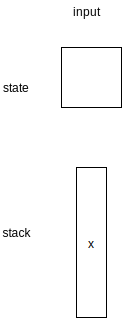
\includegraphics[scale=0.5]{Diagrams/pushdownAutomata}
\par\end{centering}
\caption{\label{fig:pushdownAutomata} Three elements control how a PDA will
compute: the input, the state, and the stack}
\end{figure}

\begin{figure}
\begin{centering}
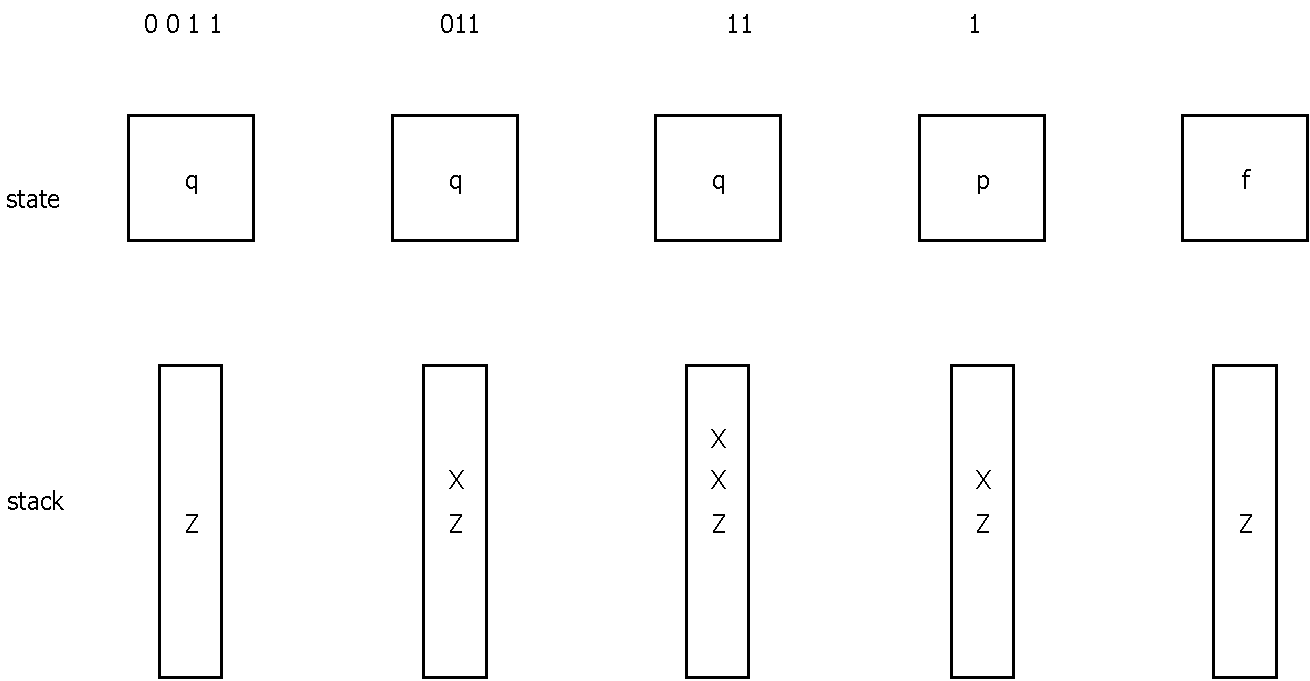
\includegraphics[scale=0.5]{Diagrams/pdaExample}
\par\end{centering}
\caption{\label{fig:pdaExample}The computation shows the evolution of the
PDA's stack, input and state as the string is processed. The initial
starting state is shown on the left and the final accepting state
is shown on the right. The following transitions define the behavior:
$\delta(q,0,Z)=\{(q,XZ)\}$, $\delta(q,0,X)=\{(q,XX)\}$, $\delta(q,1,X)=\{(p,\epsilon)\}$,
$\delta(p,1,X)=\{(p,\epsilon)\}$, $\delta(p,\epsilon,Z)=\{(f,Z)\}$}

\end{figure}


\section{Equivalence of CFG's and PDA's\label{sec:equivalenceCFGPDA}}

\subsection{Converting CFG's $\Rightarrow$ PDA's\label{subsec:Converting-CFG's-}}

For some grammar $G$, let the language $L=L(G).$ We construct the
PDA P such that upon emptying the stack we obtain a string in the
language $L$ (i.e. $N(P)=L$). P has one state $q.$ The terminals
of the grammar G become the input symbols $\Sigma$ of the PDA $P$.
The variables and terminals of G make up the stack symbols $\Gamma$
of the $P$. The start symbol of $G$ becomes the start symbol of
$P.$ Intuitively, we must model the left sentential form of a grammar
with the PDA. If the stack of the PDA $P$ is $a,$ and $P$has so
far consumed $x$from its input, then $P$ represents the left-sentential
form $xa$. 

\subsubsection{Creating the Transition Function\label{subsec:creatingTheTransitionFunction}}

There are two kinds of rules in the transition function of P, depending
on whether a terminal or variable of G is at the top of P\textquoteright s
stack. The \emph{type-1} rules handle the case where \textquotedblleft a\textquotedblright{}
is the terminal on top of P\textquoteright s stack ($\delta(q,a,a)=(q,\epsilon))$.
There better be an \textquotedblleft a\textquotedblright{} as the
next input symbol, or P has guessed wrongly about the leftmost derivation
of the input as it actually exists. In effect, we \textquotedblleft cancel\textquotedblright{}
the \textquotedblleft a\textquotedblright{} on the stack against the
\textquotedblleft a\textquotedblright{} on the input. The left-sentential
form represented does not change. We have now consumed one more symbol,
\textquotedblleft a\textquotedblright , from the input so that becomes
part of the left-sentential form. But the \textquotedblleft a\textquotedblright{}
that was on the stack is removed, so it no longer participates in
the left-sentential form. The \emph{type-2} rules handle a variable,
say $A$, on the top of the stack ($\delta(q,\epsilon,A)=(q,a))$.
We need to expand that variable by the body of one of its productions,
and thus move to the next left-sentential form. Of course we\textquoteright re
only guessing. We have to allow any of $A's$ productions to be used.
If $A\rightarrow a$ is one of these productions, then a choice for
$P$, using epsilon input, and with $A$ on top of the stack, is to
replace the $A$ by $a$.

\subsubsection{Proof of Equivalence between CFG and PDA\label{subsec:proofEquivalenceCFGPDA}}

In order to prove equivalence between the two representations we need
to prove that for all $x,$$(q,wx,S)\vdash^{*}(q,x,\alpha)\leftrightarrow S\Rightarrow_{lm}^{*}w\alpha$.
That is, for all x the instantaneous description $(q,wx,S)$ goes
to $(q,x,\alpha)$ in some number of steps of the PDA if and only
if the CFG's leftmost derivation yields $w\alpha$. It is important
to note that we allow for the suffix $x$in the string $wx$. The
string $x$ has no effect on the process of consuming $w$ and so
if the that statement is true for one $x$it is true for all $x.$
The proof follow starting from the only if direction $(\rightarrow)$.
That is, if P transitions $(q,wx,S)$ goes to $(q,x,\alpha)$, then
$S\Rightarrow_{lm}^{*}w\alpha$. This will be an inductive proof where
the base case is 0 steps have taken place and $w$ is $\epsilon$
and $\alpha$is $S$. The truth of the base case becomes trivial because
$S$ is $\alpha$ and $w\alpha$ is just $\alpha$ because $\epsilon$
serves as the identity of concatenation. Surely then, $S$ derives
itself. Now we must consider the next $n$ steps of the proof, and
assume an inductive hypothesis for the sequence of $n-1$ steps. For
the $n^{th}$ step two cases can occur. A type-1 rule is used, or
a type 2 rule is used. We will consider both case in turn. The descriptions
of these rules are described in the previous subsection. For the use
of a \emph{type-1 }rule in the $n^{th}$ step, the ID's for the 0
through $n-1$ steps must be $(q,yax,S)\vdash^{*}(q,ax,a\alpha)\vdash(q,x,\alpha)$,
where $ya=w$. That is, the prefix of the string $x$must end with
the symbol $a$ with the $a$ symbol on top of the stack followed
by $\alpha$, and in the previous $n-1$ steps the string $y$ is
consumed by the PDA, and in the $n^{th}$ step the PDA consumes the
input symbol $a$ and removes it from the stack. By the inductive
hypothesis applied to the $n-1$ steps, we can conclude that there
is a left most derivation from $S$ to $ya\alpha$ because y was consumed
and thus equivalent to $\epsilon$and $a\alpha$ is on the stack.
The symbol $a$is then consumed from the input and popped from stack
taking us back to the base case because $ya=w$. For the use of a
\emph{type-2 }rule in the $n^{th}$ step, the step sequence must be
$(q,wx,S)\vdash^{*}(q,x,A\beta)\vdash(q,x,\gamma\beta)$ where $A\rightarrow\gamma$
is a production in the grammar and $\alpha=\gamma\beta$. In this
case, we have a variable $A$ on top of the stack followed by the
stack string $\beta$. In the $n^{th}$ step no input is consumed
but the variable $A$ is replaced by the stack string $\gamma$. By
the inductive hypothesis we obtain $S\Rightarrow_{lm}^{*}wA\beta$
after the first $n-1$ steps. Because $A$ is the leftmost variable
in the derivation it is replaced by $\gamma$. We then have $S\Rightarrow_{lm}^{*}w\gamma\beta=w\alpha$
returning us to our base case, thus proving the only if direction
of the proof. Next, we prove the if direction ($\leftarrow)$. We
now must prove $S\Rightarrow_{lm}^{*}w\alpha\rightarrow(q,wx,S)\vdash^{*}(q,x,\alpha)$
for all $x$ $\ldots${[}omitted{]}

\subsection{Converting PDA's $\Rightarrow$ CFG's\label{subsec:convertingPDA2CFG}}

In this section we obtain the grammar $G$ from a PDA $P$. We assume
that the language $L$ is accepted by the PDA upon emptying its stack,
more formally $L=N(P).$ Intuitively, we should assign variables labeled
as $pXq$ to the grammar $G$ for the transitions from state $p$to
state $q$when popping the symbol $X$ from the PDA's stack. Upon
popping the $X$ from the stack it may grow, but the stack size will
not shrink below the size when $X$ was popped off the stack until
the last step in processing is taken.

\subsubsection{Constructing Variables of the CFG\label{subsec:constructingVariablesOfCFG}}

The variables of $G$ are correspond to labels such as $pXq$ which
can be viewed as a single symbol modeling the transition from p to
q with X on the stack in which the input is consumed and generates
all and only the strings $w$ until $\left(p,w,X\right)\vdash^{*}(q,\epsilon,\epsilon)$.
Note that since the initial ID shows nothing below $X$ on the stack,
we know that $X$ can\textquoteright t be popped until the last step,
since PDA P cannot make any moves when its stack is empty.In addition
to the aforementioned variable a start symbol $S$ is needed.

\subsubsection{Constructing Productions of the CFG\label{subsec:constructingProductionsOfCFG}}

Intuitively, the productions or rules of the grammar represent steps
of the PDA. Each rule for the example rule $pXq$ is sourced from
the PDA in state $p$with the stack symbol $X$. In the easiest case
we have the following for the PDA's transition function. $\delta(p,a,X)$
yields $(p,\epsilon)$. Here $a$ denotes either a input symbol or
$\epsilon$. The grammar in this case can model the PDA's behavior
by popping $X$and not replacing it with any other symbol $(pXq\rightarrow a)$.
The next simplest case simplest case involves modeling transition
between productions. Transitivy is modeled by introducing an intermediate
state $r$and a variable $Y$. The transition function in this case
would look like $\delta(p,a,X)$ yields $(r,Y)$. The corresponding
production would then be $pXq\rightarrow arYq$. This allows us to
erase X and transition from $p$ to $q$ by way of $r$ while reading
$a$and pushing $Y$ onto the stack. The final simplest case we will
consider is $\delta(p,a,X)$ yields $(r,YZ)$ for some state $r$
and some symbols $Y$and $Z$. Here $X$ is replaced by $YZ$. In
order for $X$ to be erased, there must be some input string u that
has the net effect of erasing $Y$. And $u$ must take the PDA from
state $r$ to some state $s$, which we don\textquoteright t know.
As a result, we\textquoteright re going to have to have one production
for each state $s$. But after reaching state $s$, we must have some
additional input $v$ that takes the PDA from state $s$ to state
$q$, while popping the $Z$ from the stack. The net effect is that$auv$
pops $X$ from the stack while going from state $p$ to $q.$ The
general case for creating productions to model the PDA follows. Suppose
$\delta(p,a,X)$ yields $(r,Y_{1},\ldots Y_{k})$ for some state $r$
and $k\geq3.$ Then in the grammar generate the set of productions
$pXq\rightarrow arY_{1}s_{1}s_{1}Y_{2}s_{2}\ldots s_{k-2}Y_{k-1}s_{k-1}s_{k-1}Y_{k}q$.
This models the case in which $X$ is replaced by three or more symbols
transitioning from $p$ to $q.$

\section{Pumping Lemma for Context Free Languages\label{sec:pumpingLemmaForContextFreeLanguages}}

Recall the concepts for the pumping lemma on regular languages outlined
in Section\vref{sec:pumpingLemmaRegularLanguages}. The pumping lemma
for regular languages relied on a cycle early on in a sufficiently
long string $w$ in order ``pump'' an the string an arbitrary number
of times, thus producing a infinite number of strings in the language.
Similarly, the pumping lemma for context free languages models this
idea, but requires two cycles along the string's path in tandem. 

\subsection{Formal Specification of the CFL Pumping Lemma\label{subsec:formalSpecificationOfContextFreeLanguages}}

For every context free language $L$, there is an integer $n$, such
that for every string $z$ in $L$ of length $\geq n$ there exists
$z=uvwxy$ such that the following conditions hold:
\begin{enumerate}
\item $|vwx|\leq n.$
\item $|vx|>0.$
\item For all $i\geq0$, $uv^{i}wx^{i}y$ is in $L.$
\end{enumerate}
If a language in question does not have these properties, then it
is not a context free language.

\section{Properties of Context Free Languages\label{sec:propertiesOfContextFreeLanguages}}

\subsection{Decision Properties of Context Free Languages\label{subsec:decisionPropertiesOfContextFreeLanguages}}

Like regular languages we can determine many decision properties about
context free languages including whether a string in the particular
CFL, whether a CFL contains any strings at all, and if the CFL contains
an infinite number of strings. Unfortunately,we cannot decide whether
two CFL's are equivalent, or whether they are disjoint.

\subsubsection{Membership Test for CFL's\label{subsec:membershipTestForCFL}}

The membership test is used to determine whether a given string $w$
is the language of the grammar $L(G).$ We need the grammar to be
in Chomsky Normal Form, so if it isn't then convert it to this form
as described in subsection\vref{subsec:representingGrammarsInChomskyNormalForm}.
Then use the CYK algorithm to determine the status of $w.$ The CYK
algorithm uses Dynamic Programming to decide whether $w$ is in the
language or not, so it may be useful to first review the section\vref{sec:Dynamic-Programming}
first in order to gain better understanding of CYK.

\subsubsection{The CYK Algorithm}
\begin{flushleft}
Let $w=a_{0}\ldots a_{n}$ be a string of length $n$where $a_{i}$
stores the symbol at the $i^{th}$ position. Construct a $n$ by $n$
triangular array. This can done efficiently by using an indexing function
where upon a single-indexed array is mapped to an upper-triangular
array. The following function $k=j(j+1)/2+i$ where $k$ represents
the index into the array properly maps the elements of the array.
This idea can be viewed in Figure\vref{fig:triangularArray}. Additionally,
each entry of the array should be viewed as a set of variables of
the grammar. The set $X_{ij}$ is stored in position $(i,j)$ of the
array where $i\leq j$ and is intended to be the set of variables
that derive the substring of the input starting from position $i$
and ending at position $j$. An inductive argument is used to fill
the table on the length of the input string derived . The length of
the string can be computed as $j-i+1$. We start by computing the
entries $X_{i,i}$, which is the set of variables that derive the
string consisting of the symbol at $a_{i}$ . Next, we find the variables
at $X_{i,i+1}$ each of which derive the string at $a_{i,i+1}$. Then,
we move to the $X_{i,i+2}$ variables which are the sets of variables
that derive the strings of length three, $a_{i},$$a_{i+1},$$a_{i+2}$
and so on . Finally, after we have computed the set $X_{1,n}$ which
represents the entire input string , we can test whether the start
symbol $S$ is contained in the set . If it is then the string is
in the language, otherwise it is not. Formally, the basis $X_{i,i}=\{A|A\Rightarrow^{*}a_{i}\}$
where $a_{i}$ represents a single symbol in $w$. The induction is
then $X_{i,j}$=\{A| there is a production $A\rightarrow BC$, and
an integer $k$, with $i\leq k<j$, such that $B$ is in $X_{i,k}$
and $C$ is in $X_{k+1,j}$\}.That is, for each $k$ between $i$
and $j-1$ we look for some $B$ in $X_{i,k}$ and some $C$ in $X_{k+1,j}$
such that $BC$ is the body of an $A$ production. If for any $k$,
$B$, and $C$ we find such a production, we add $A$ to $X_{i,j}$.
\begin{figure}
\begin{centering}
\begin{tabular}{r@{\extracolsep{0pt}.}lr@{\extracolsep{0pt}.}lr@{\extracolsep{0pt}.}lr@{\extracolsep{0pt}.}l}
\multicolumn{2}{c}{0} & \multicolumn{2}{c}{1} & \multicolumn{2}{c}{3} & \multicolumn{2}{c}{6}\tabularnewline
\multicolumn{2}{c}{} & \multicolumn{2}{c}{2} & \multicolumn{2}{c}{4} & \multicolumn{2}{c}{7}\tabularnewline
\multicolumn{2}{c}{} & \multicolumn{2}{c}{} & \multicolumn{2}{c}{5} & \multicolumn{2}{c}{8}\tabularnewline
\multicolumn{2}{c}{} & \multicolumn{2}{c}{} & \multicolumn{2}{c}{} & \multicolumn{2}{c}{9}\tabularnewline
\end{tabular}
\par\end{centering}
\centering{}\caption{\label{fig:triangularArray}A single index array can be viewed as
a triangular array by accessing it with a function mapping the rows
and columns appropriately. The function $k=j(j+1)/2+i$ maps the index
value $k$ to the appropriate $i$ and column $j$ where $i\leq j$.}
\end{figure}
\par\end{flushleft}

\subsubsection{Emptiness Test for CFL's\label{subsec:emptinessTestForCFL}}

The algorithm to test for an empty CFL uses the ideas we learned in
subsection\vref{subsec:eliminatingUselessVariables}. We use these
ideas of checking whether variables are useful in the derivation to
determine if the start symbol $S$ is a useful symbol. If the start
symbol does not derive anything, it is a useless variable, and we
can state that the CFL is empty. 

\subsubsection{Infiniteness Test for CFL's\label{subsec:infinitenessTestCFL}}

The test for infinteness in CFL mirrors the idea that was proposed
in section\vref{subsec:infinitenessTestRegularLanguages}. Apply those
principles with the pumping lemma for context free languages outlined
in section\vref{sec:pumpingLemmaForContextFreeLanguages}.

\subsection{Closure Properties of Context Free Languages\label{subsec:closurePropertiesOfContextFreeLanguages}}

For many of the same operations under which the class of regular languages
are closed, the context-free languages are also closed. These include
the regular-expression operations: union, concatenation, and closure.
Also reversal, homomorphism and inverse homomorphism. But unlike the
class of regular languages, the class of context-free languages is
not closed under intersection or difference. 

\subsubsection{Union for CFL's\label{subsec:unionForCFL's}}

//TODO

\subsubsection{Concatenation for CFL's\label{subsec:concatentationForCFL's}}

//TODO

\subsubsection{Kleene Closure for CFL's\label{subsec:kleeneClosureForCFL's}}

//TODO

\section{Countability\label{sec:Countability}}

It is important to understand that all computation can be encoded
as integers. The ASCII or if you like the UTF-8 table encodes English
characters and algebraic numerals, which we can interpret as integers.
This idea can be applied to all types of media. At the very root we
may interpret all things as integers.

\subsection{Finite Sets}

A finite set is a set that contains a finite number of elements. Refer
to Section\vref{sec:Sets}. It may be useful to refresh your memory
on this topic. The formal definition of a finite set is one for which
it is impossible to find a one to one correspondence between the members
of the set and a proper subset of the set. An example of a set is
$\{a,b,c\}.$

\subsection{Infinite Sets}

An infinite set is a set for which there is a one to one correspondence
between itself and a proper subset of itself. An example of a infinite
set is the positive integers $\{1,2,3,\ldots\}.$ The one-to-one correspondence
which validates this argument is the mapping of the positive integers
with the even integers ( $1\leftrightarrow2,2\leftrightarrow4,3\leftrightarrow6,\ldots)$.

\subsection{Countable Sets}

A countable set is a set with a one to one correspondence with the
positive integers, thus all countable sets are infinite sets. As another
example all integers $\mathbb{Z}$ form a countable set. 0 is mapped
to 1 and the negative integers are are mapped to the even numbers
($-i\leftrightarrow2i$, for all $i\geq1$), while the positive integers
are mapped to odd numbers$(i\leftrightarrow2i+1$, for all $i\geq1$).
The enumerated sequence then becomes $0,-1,1,-2,2,-3,3,\ldots$ Another
example of an enumerable set is the binary strings, but there is a
trick involved. The binary strings $101,0101,00101$ all correspond
to the integer value 5, so it seems impossible to form a correspondence
such that they become countable. The trick here is to prepend a 1
to the binary strings so that the strings can become distinguishable.
The aforementioned strings become $1101,10101,100101$ as integers
they are 13, 21, and 37.

\subsection{Countability of Languages Over the Binary Alphabet}

The next bit is quite confusing (pun intended). The languages over
the binary alphabet $\Sigma=\{0,1\}$ are not countable. To obtain
a contradiction we use a technique that confounds a set formers specification.
As with the other examples suppose we could encode languages over
the binary alphabet so that we could speak about some specific enumerated
language. For example, the $i^{th}$ language. Define the language
$L$ = \{ w | w is the $i^{th}$ binary string and $w$ is not in
the $i^{th}$ language\}. Surely, the language $L$ is a language
over the binary alphabet. Thus, $L$ is the $j^{th}$ language for
some particular $j.$ Now let some binary string $x$be the $j^{th}$
string. Now consider substituting $x$for $w$ in the $j^{th}$ language
$L_{j}$ = \{ $x$ | $x$is the $j^{th}$ binary string and $x$is
not in the $j^{th}$ language\}. For some arbitrary $j^{th}$ string
$x$in the $j^{th}$ language $L_{j}$, if $x$is in $L_{j}$, then
it cannot be by the definition of the language. If $x$is not in the
language $L_{j}$, then $x$is in the language by the definition of
the language. This makes for a very confusing situation. Remember,
$L$ contains $w$ if and only if $w$ is not the language that corresponds
to the same integer $i$ that $w$ corresponds to. We now have a contradiction
and therefore we know that we know the languages over the binary strings
are not countable. Graphically, this concept can be seen in the Diagonalization
Method in Figure\vref{fig:diagonalization}.

\begin{figure}
\begin{centering}
\begin{tabular}{cc|c|c|c|c|c|c|}
 & \multicolumn{1}{c}{} & \multicolumn{6}{c}{Strings}\tabularnewline
 & \multicolumn{1}{c}{} & \multicolumn{1}{c}{1} & \multicolumn{1}{c}{2} & \multicolumn{1}{c}{3} & \multicolumn{1}{c}{4} & \multicolumn{1}{c}{5} & \multicolumn{1}{c}{$\ldots$}\tabularnewline
\cline{3-8} 
\multirow{6}{*}{Languages} & 1 & 1 & 0 & 1 & 1 & 0 & \tabularnewline
\cline{3-8} 
 & 2 &  & 1 &  &  &  & \tabularnewline
\cline{3-8} 
 & 3 &  &  & 0 &  &  & \tabularnewline
\cline{3-8} 
 & 4 &  &  &  & $\ddots$ &  & \tabularnewline
\cline{3-8} 
 & 5 &  &  &  &  &  & \tabularnewline
\cline{3-8} 
 & $\vdots$ &  &  &  &  &  & \tabularnewline
\cline{3-8} 
\end{tabular}
\par\end{centering}
\caption{\label{fig:diagonalization} This diagram depicts a table used to
describe whether strings are in a language or not. A binary integer
1 indicates that the string $j^{th}$ string is in the $i^{th}$ language,
0 indicates it is not in the language. Look at the diagonal in this
table. If you were to first complement the main diagonal and then
rotate it by 45 degrees upon an axis created in the $i^{th}$ row
and $i^{th}$ column, then it too would look like a language, but
would always disagree with itself at the $i^{th}$ row and $i^{th}$
column.}

\end{figure}


\section{Turing Machines\label{sec:Turing-Machines}}

Turing machines model the recursively enumerable languages which encompass
the previously discussed languages. Sipser provides a good hierarchy
to reference for how to regard which language classes are subsets
of which. The diagram is provided in Figure\ref{fig:languageClassHierarchy}.
The purpose of Turing Machine theory is to provide a means of proving
whether or not an algorithm exists for a given language.Reductions
which will be explored in detail in later sections prove common questions
are undecidable. 

\begin{figure}
\begin{centering}
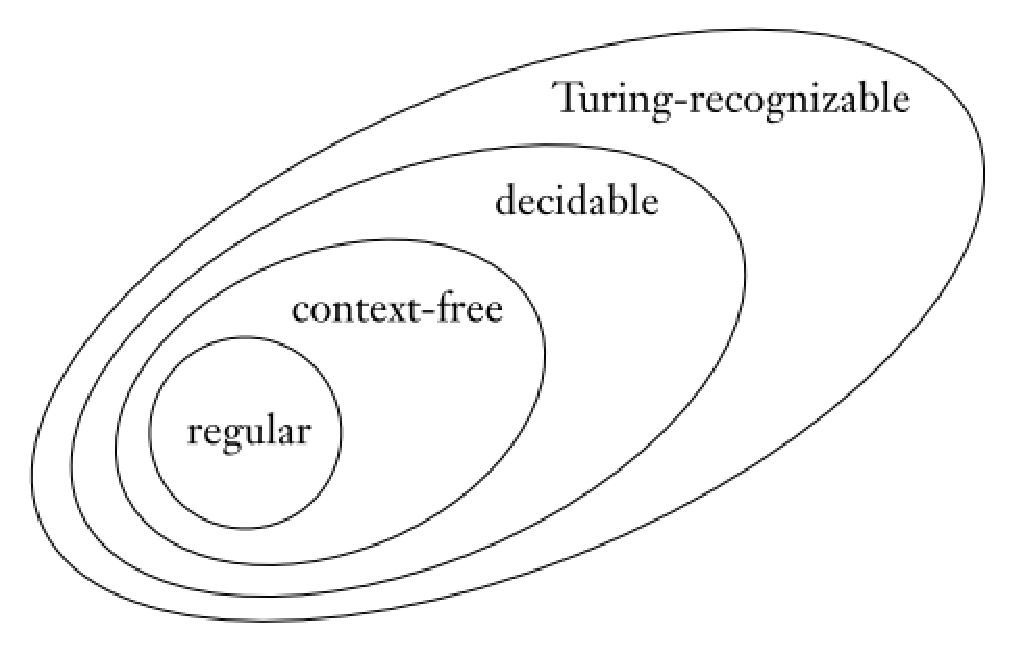
\includegraphics[scale=0.5]{Diagrams/LanguageClassHierarchy}
\par\end{centering}
\caption{\label{fig:languageClassHierarchy} The hierarchy of language classes.
Turing-recognizable languages are sometimes called recursively enumerable
languages. Decidable languages are sometimes called recursive languages.}

\end{figure}


\subsection{What is a Turing Machine?}

A Turing Machine is a computational model composed of a tape and a
head that reads and writes symbols onto the tape based on a transition
function. The tape is infinite in both directions, and there is also
some state that we track throughout computation. In one step of computation
the Turing machine may read one symbol from the tape and modify it,
and either move the head left or right one square.

\subsection{Turing Machine Notation}

A Turing machine is made up of the following components.
\begin{itemize}
\item A finite set of states ($Q).$
\item An input alphabet $(\Sigma).$
\item A tape alphabet $(\Gamma,$typically $\Sigma\subseteq\Gamma)$.
\item A transition function ($\delta$).
\item A start state ($q_{0}\varepsilon Q)$.
\item A blank symbol ($\sqcup\subseteq\Gamma-\Sigma).$
\item A set of final states ($F\subseteq Q)$.
\end{itemize}
Conventionally, the lowercase letters at the beginning of the alphabet
are input symbols ($a,b,c).$ Upper case letters at the end of the
alphabet represent tape symbols $(X,Y,Z)$. Lowercase letters at the
end of the alphabet represent input strings $w,x,y,z$. Greek symbols
represent tape symbols $(\alpha,\beta,\gamma)$. The transition function
$\delta$ takes two parameters a $q_{i}\varepsilon Q$ and a tape
symbol in $\Gamma$. The transition function yields a triple of the
form (state, tape symbol, direction). If for a given input a transition
is not defined then the Turing machine halts in the current state.

\subsection{Instantaneous Descriptions of Turing Machines}

Instantaneous descriptions of Turing Machines are encoded as $\alpha q_{i}\beta$
where $\alpha$ represents the tape before the head of the Turing
Machine until the leftmost blank and $\beta$ represents the tape
after the head until the rightmost blank. The position of the head
represented by a state symbol $q_{i}$ is just left of the tape string
$\beta$. Further we use the symbol $\vdash$ to indicate ``becomes
in one move'' and $\vdash^{*}$ as ``becomes in zero or more moves.'' 

\subsection{Languages of a Turing Machine}

A Turing machine's language is defined by its final states or a halting
action. An example is $L(M)$ = \{ $w$ | $q_{0}w\vdash^{*}I$ , where
I is an ID with a final state\}. Halting can be described by $H(M)$
= \{$w$ | $q_{0}w\vdash^{*}I$, and there is no move possible from
$I\}.$

\subsection{Recursively Enumerable Languages vs. Recursive Languages}

The class of languages accepted by a Turing Machine halting or entering
an accepting state is called the Recursively Enumerable language class.
Some textbooks also call this the Turing Recognizable language class.
Turing Machines that accept by final state, and who are \emph{guaranteed
to halt} whether it accepts or not define the Recursive Languages
class. In some textbooks this is called the Decidable Language class. 

\subsection{Multi-tape Turing Machines}

Multi tape Turing Machines allow for a ordinary Turing Machine to
have $k$ tapes for any fixed $k.$ The steps the Multi tape Turing
Machine makes are dependent on the symbols the head of each tape is
pointing to and their corresponding states. Each tape has its own
head and they move on their own tape without restricting each others
movement. On each read of the tape a new symbol and state is assigned
for each tape and head. Additionally, a head may choose to not move.
This model is no more powerful than the traditional Turing Machine.
One may simply expand the alphabet for a traditional Turing Machine
to accommodate the number of tapes that it must simulate.

\subsection{Nondeterministic Turing Machines}

Nondeterministic Turing Machines are granted multiple choices based
on the state, direction, move triple. Once a choice is made, then
the next state, new symbol and head direction are determined. As with
the NFA's, DFA's, and PDA's, the nondeterministic Turing Machine accepts
if any sequence of choices leads to an ID with and accepting state.

\subsection{Closure Properties of Recursive and Recursively Enumerable Languages}

Recursive Languages and Recursively Enumerable Languages share the
properties: union, concatenation, Kleene star, reversal, intersection,
and inverse. Recursive languages have difference and complementation.
Recursively Enumerable Languages have homomorphism.

\begin{figure}
\begin{centering}
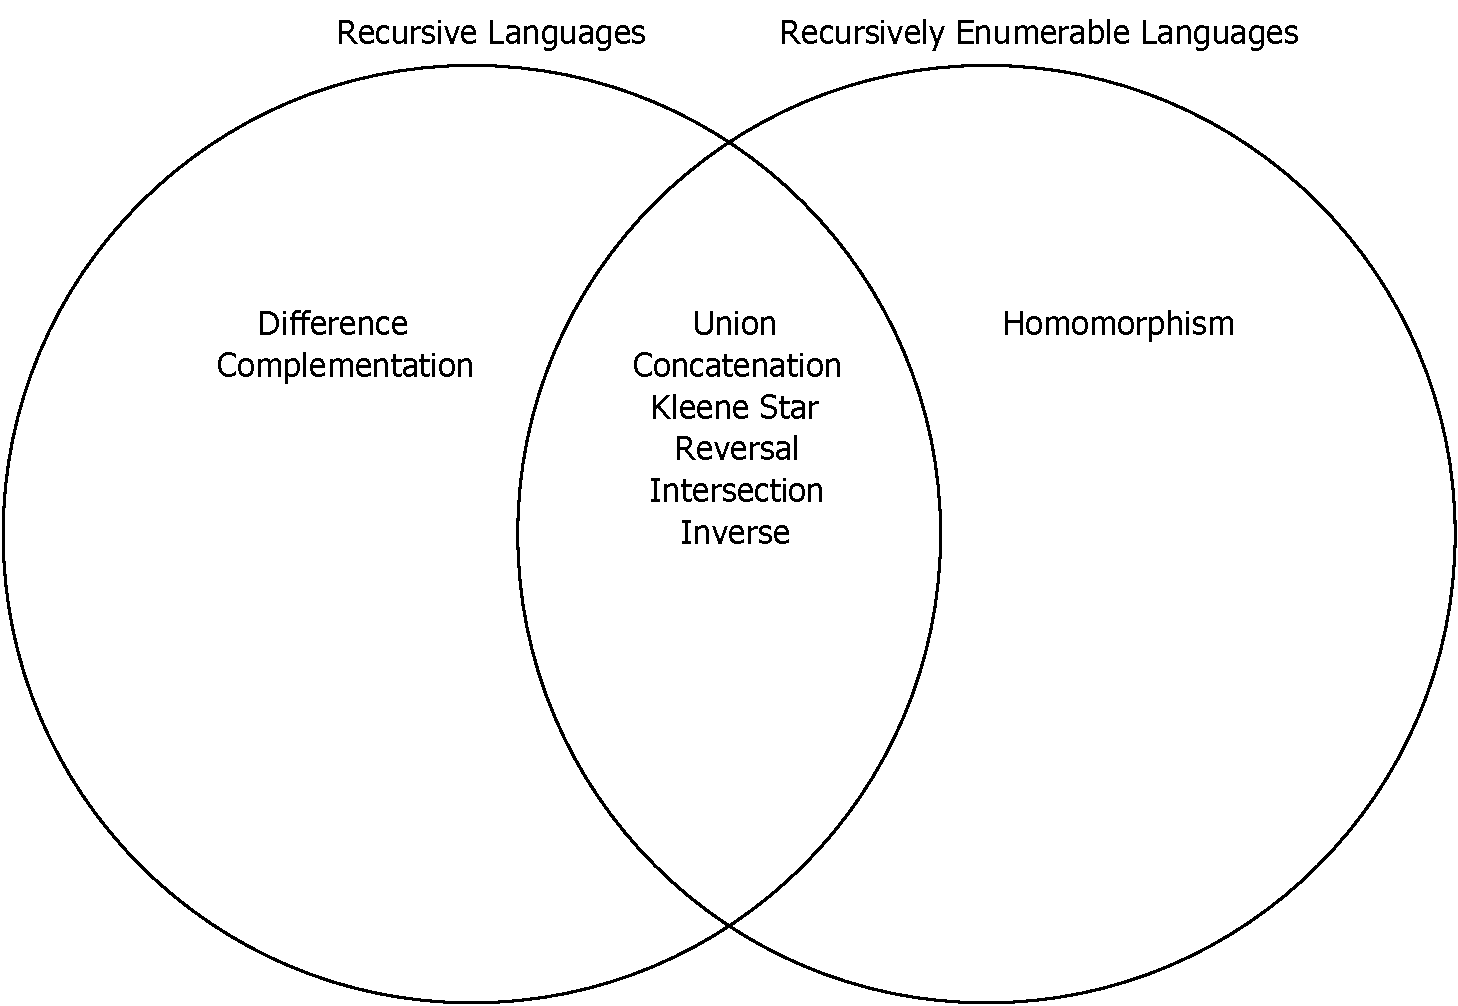
\includegraphics[scale=0.5]{Diagrams/ClosurePropertiesRELandRL}
\par\end{centering}
\caption{\label{fig:closurePropertiesOfRELandRELanguages}The closure properties
of Recursive and Recursively Enumerable languages}
\end{figure}


\subsubsection{Union}

Given two Turing machines $M_{1}$ and $M_{2}$ with languages $L_{1}$and
$L_{2}$ respectively. The union of $M_{1}$ and $M_{2}$ can be achieved
by creating a third Turing Machine $M$. $M$will be a two-tape Turing
Machine. $M$ will proceed by copying the tape of $M_{1}$ to its
first tape, and $M_{2}$ to its second tape. Next, $M$ will simulate
the input of $M_{1}$ and $M_{2}$ independently. In the case of Recursive
Languages (Decidable Languages), $M$will \emph{accept} when either
of its tapes enter an accepting state, and \emph{reject} when \textbf{both}
of its tapes halt by not accepting. The case for Recursively Enumerable
Languages is a bit more relaxed. In this case, $M$ need only to enter
an accepting state on one of its tapes to accept. However, it may
end up running forever and never providing an answer. 

\subsubsection{Intersection}

The idea behind intersection is quite similiar to union. Given two
Turing machines $M_{1}$ and $M_{2}$ with languages $L_{1}$and $L_{2}$
respectively. The intersection of $M_{1}$ and $M_{2}$ can be achieved
by creating a third Turing Machine $M$. $M$will be a two-tape Turing
Machine. $M$will proceed by copying the tape of $M_{1}$ to its first
tape, and $M_{2}$ to its second tape. Next, $M$ will simulate the
input of $M_{1}$ and $M_{2}$ independently. In the case of Recursive
Languages (Decidable Languages), $M$will \emph{accept} when \textbf{both}
of its tapes enter an accepting state, and \emph{reject} when \textbf{either}
of its tapes halt by not accepting. In the Recursively Enumerable
case, $M$ has to enter an accepting state on \textbf{both} of its
tapes to accept. However, it may end up running forever and never
provide an answer. 

\subsubsection{Difference and Complement}

Again the idea behind Difference and Complement is quite similiar
to the intersection. The intersection of $M_{1}$ and $M_{2}$ can
be achieved by creating a third Turing Machine $M$. $M$ will be
a two-tape Turing Machine. $M$ will proceed by copying the tape of
$M_{1}$ to its first tape, and $M_{2}$ to its second tape. Next,
$M$ will simulate the input of $M_{1}$ and $M_{2}$ independently.
$M$ will \emph{accept} when \textbf{$M_{1}$ }accepts and $M_{2}$
rejects, otherwise reject. Corollary, for the complement run the difference
algorithm over the Kleene star of the input alphabet. This approach
won't work for Recursively Enumerable Languages because $M_{2}$ may
never halt.

\subsubsection{Concatenation}

Concatenation will require the use of a two-tape nondeterministic
Turing Machine $M$. Assume that the given machines $M_{1}$ and $M_{2}$
are semi-inifinite single-tape Turing Machines. $M$ will proceed
by nondetminitically guessing the where a given input string $w$
should be split. Call the prefix substring of $w$ the string $x$,
and call the corresponding suffix $y$. Now copy $x$ onto $M's$
first tape and $y$onto its second tape. Now simulate $M_{1}'s$ transition
function on the first tape and $M_{2}'s$ transtion function on the
second tape. If both accept then $M$ should \emph{accept}, otherwise
\emph{reject}. Because we nondeterministically guess all ways that
$w$ can be split the machine will always accept if $w$ is in $L(L(M_{1})L(M_{2})).$ 

\subsubsection{Kleene Star}

For the Kleene star mirror the technique of used concatenation but
instead of splitting the input string. Generate the Kleene star of
the given Turing Machine and for each component of the guessed set
run it against the Turing Machine and if it accepts then accept, otherwise
reject.

\subsubsection{Reversal}

Simply reverse the input and run it against the machine.

\section{Decidability\label{sec:Undeciability}}

Now that we have seen some algorithms in the preceeding section it
is easy to see that one may create a great number of algorithms for
Turing Machines. However, we will soon find out that for some problems
no algorithm exists. We will link the concepts we learned in the Section\vref{sec:Countability}
to formulate a way of encoding Turing Machines in binary. This will
allow us to apply the Diagonalization technique to Turing Machines.
We can then formalize the notion that a problem posed to a Turing
Machine is in fact the language of the Turing Machine. We can then
see that for some languages no Turing Machine can exist.

\subsection{Encoding Turing Machines in Binary}

It is quite simple to come up with a scheme for encoding Turing Machines
into binary strings. We will assume the Turing Machines we will be
encoding have a input alphate consisting of $\{0,1\}.$ However, this
methodology is certainly exapandable to arbitrary alphabets. We should
first assign integer values to the three classes of elements of the
Turing Machine: states, symbols, and directions. Now we apply a trick
for distinguishing codes of the binary string. For each integer representation
of the componenet. Convert the integer to binary and insert a zero
for each binary digit. Now there can never be consecutive ones in
the binary representation. To distinguish between parts of the encoding
add consecutive ones. Now we can concatenate the elements of the Turing
machine together and prepend a 1 so that the encoding represents a
unique integer value, and thus the language of all possible Turing
Machines becomes enumerable. Some encodings may give invalid Turing
Machines and therefore we regard theses as Turing Machines that accpet
only the empty language.

\begin{figure}
\begin{centering}
\begin{tabular}{cc|c|c|c|c|c|c|c|c|}
 & \multicolumn{9}{c}{String j$\rightarrow$}\tabularnewline
\multirow{9}{*}{TM i$\rightarrow$} & \multicolumn{1}{c}{} & \multicolumn{1}{c}{1} & \multicolumn{1}{c}{2} & \multicolumn{1}{c}{3} & \multicolumn{1}{c}{4} & \multicolumn{1}{c}{5} & \multicolumn{1}{c}{6} & \multicolumn{2}{c}{$\ldots$}\tabularnewline
\cline{3-10} 
 & 1 & $a_{1,1}$ &  &  &  &  &  &  & \tabularnewline
\cline{3-10} 
 & 2 &  & $a_{2,2}$ &  &  &  &  &  & \tabularnewline
\cline{3-10} 
 & 3 &  &  & $a_{3,3}$ &  & x &  &  & \tabularnewline
\cline{3-10} 
 & 4 &  &  &  & $a_{4,4}$ &  &  &  & \tabularnewline
\cline{3-10} 
 & 5 &  &  &  &  & $a_{5,5}$ &  &  & \tabularnewline
\cline{3-10} 
 & 6 &  &  &  &  &  & $a_{6,6}$ &  & \tabularnewline
\cline{3-10} 
 & \multirow{2}{*}{$\vdots$} &  &  &  &  &  &  & $\ddots$ & \tabularnewline
\cline{3-10} 
 &  &  &  &  &  &  &  &  & \tabularnewline
\cline{3-10} 
\end{tabular}
\par\end{centering}
\caption{\label{fig:TuringMachineAcceptanceTable}This table expreses which
strings $j$ are accepted by which Turing Machines $i$. If $x$is
0 then the string is not accpeted, otherwise if 1 then it is accepted.
The main diagonal $D$ is enumerated as $a_{1,1},a_{2,2},a_{3,3},\ldots,a_{n,n}$. }

\end{figure}


\subsection{Diagonalization on the Enumerated Turing Machines\label{subsec:DiagonalizationOnTuringMachines}}

In order to diagonalize the table given by Figure\vref{fig:TuringMachineAcceptanceTable}.
We form a sequence $D$ by complementing the values along the main
diagonal. Formally $D=$$a_{i,j},\ldots,a_{n,n}$ where $i=j$, and
the value of $a_{i,j}$ is the complement of its value in the table
shown in Figure\vref{fig:TuringMachineAcceptanceTable}. Now we come
to the question: Could $D$ be a row representing the language accepted
by a Turing Machine of the table? Suppose this imaginary row represented
by the main diagonal $D$ where row $k$, but it can't be row $k$
because it disagrees at the $k^{th}$ entry. Therefore this cannot
be the language of any Turing Machine, and further we can descibe
this language as the set that contains the $k^{th}$ string if and
only if the $k^{th}$ Turing Machine does not accept the $k^{th}$
string. We can name this language $L_{D}$ and since we know that
we can not create a Turing Machine for this langauge, then we know
that it is not recursively enumeable (Turing-recogizable), and thus
no algorithm can be given to decide $L_{D}.$

\subsection{Decidable Problems}

A problem is decidable if there is an algorithm to asnwer it. Recall,
an algorithm formally speaking is a Turing Machine that halts on all
inputs, accepted or not. Put another way a deciable problem is a recursive
language. We may visualize the relationship among the language classes
and the language $L_{D}$ which we identified in subsection\vref{subsec:DiagonalizationOnTuringMachines}
in the Figure

\begin{figure}
\begin{centering}
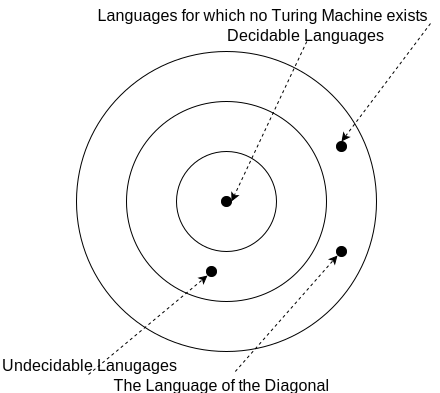
\includegraphics[scale=0.5]{Diagrams/DecidablityLanguageClass}
\par\end{centering}
\caption{\label{fig:DeciableLanguagesDiagram} Here we see the hierarchy of
the language classes and how they relate to $L_{D}$. The Undeciable
Languages also called the Recursively Enumerable Languages have a
Turing Machive and are regarded to be Turing-recognizable. That is,
they have a Turing Machine that will accept strings, but there is
no guarantee that the machine will halt. Within this class is the
Decidable Languages also called the Recursive Languages which have
Turing Machines which are guranteed to distinguish string as either
accepted or rejected and they also are guranteed to halt. At the otter
most ring we have the language for which no Turing Machine exists
and therefore they are unrecognizable.}

\end{figure}


\subsection{The Universal Turing Machine}

A Universal Turing Machine (UTM) is a Turing Machine which accepts
as input a Turing Machine $M$ and some string $w$. The UTM accepts
$M$ if and only if $M$accepts $w.$ A UTM will have three tapes.
Tape 1 holds the input $M$encoded as binary and $w.$ Tape 2 holds
the tape of $M$, and Tape 3 holds the state of $M.$ The UTM proceeds
by first checking the encoding of $M.$ If $M$ is invalid, then its
language is the empty language, and the UTM halts immediately and
rejects. The UTM will then examine the size of $M's$ symbols to determine
the required word size. Next, the UTM will initialize Tape 2 to represent
the tape of $M$with the input $w$, and initialize Tape 3 to hold
the start state. Finally, the UTM can simulate $M$ by looking for
a step in the transition function of $M$encoded on Tape 1 that matches
the state encoded on Tape 3 with a tape symbol under the head of Tape
2. If a match is found change the symbol and move the head marker
on Tape 2 and change the State on Tape 3. If $M$accepts, then the
UTM accepts.

\subsection{The UTM is Recursively Enumerable and Not Recursive (The Halting
Problem)\label{subsec:haltingProblem}}

Assume for the purposes of contradiction that the language of the
UTM, that is $L(UTM)$, is recursive (decidable). Meaning that for
every input it halts and returns an accepting or rejecting answer.
We \emph{somehow magically discover} an algorithm that can decide
whether given a Turing Machine$M$ and an input string $w$ from the
acceptance table featured in Figure\vref{fig:TuringMachineAcceptanceTable}\textendash{}
call this algorithm \emph{wizzBang. }Remember \emph{wizzBang }takes
two paramters as arguments. First, we must have a valid Turing Machine
$M$, and second we must have a string $w.$ We\textquoteright re
given an input $M$. Let\textquoteright s suppose $M$ is for the
i-th string $w$ of our table. The first thing to do is check whether
or not $M$ is a valid encoding for a Turing machine. If the encoding
is NOT valid, then the i-th Turing Machine defines the empty language.
That means $w$, the i-th string, is not in the language of the i-th
Turing machine. Therefore, $w$ IS in $L_{D}$. Remeber we complemented
the major diagonal so that answers here must be inverted. Now suppose
$M$ is a valid encoding for a Turing machine. Then run \emph{wizzBang}
on the input $M$ and $w$. Here $M$ represents the i-th Turing Machine
processing the input that is the i-th string. Eventually, this algorithm
will halt and tell us whether or not the i-th machine accepts the
i-th string. If the \emph{wizzBang} accepts the i-th machine accepts
the i-th string, then we say reject because that means $w$ is not
in $L_{D}$. However, if \emph{wizzBang} rejects, then we accept $w$,
because $w$ IS in $L_{D}$. HERE IS THE MAIN POINT$\Rightarrow$
We previously proved in subsection\vref{subsec:DiagonalizationOnTuringMachines}
that no Turing Machine can exist for $L_{D}$ and therefore we must
conclude that \emph{wizzBang cannot exist. }This tells us that the
UTM is Recursively Enumerable (Turing-recognizable), but not Recursive
(Decidable). We will regard the language of the UTM as $L_{U}$ going
forward.

\section{Some Undeciable Problems}

In this section we cover Rice's Theorem which states that almost every
question we ask about Recursively Enumerable Languages is undeciable.
Next we look to Post's Correspondence Problem to bridge the gap between
the world of Turing Machine to solving real world problems. In addition
to the classical language classes we have defined we may define properties
of languages. A property is a user defined set of languages. For example,
the set of languages who are infinite languages have the Infiniteness
Property. We can define a language $L_{P}$ as the set of TM's such
that each TM has the property $P$. There are two trivial propertues
$P$ for which $L_{P}$ is deciable. The always-false propety, which
contains no Recursively Enumerable languages, and the always-true
property, which contains every Recursively Enumerable language. Rice's
Theorem states that for every other property $P$ besides the trivial
ones $L_{P}$ is undecidable. In order to prove Rice's Theorem we
will have to introduce the concept of reductions. A reduction is an
algorithm (Recall, an algorithm is a TM that always halts), which
transforms an input string $w$ in $L$ to a string $x$in $L'$ with
the property that $x$is in $L'$ if and only if $w$ is in $L.$
The takeaway here is that given the reduction for $L$ we are able
to say that $L$ is no harder than $L'.$ We can visualize reductions
as shown in Figure\vref{fig:Reductions}.

\begin{figure}
\begin{centering}
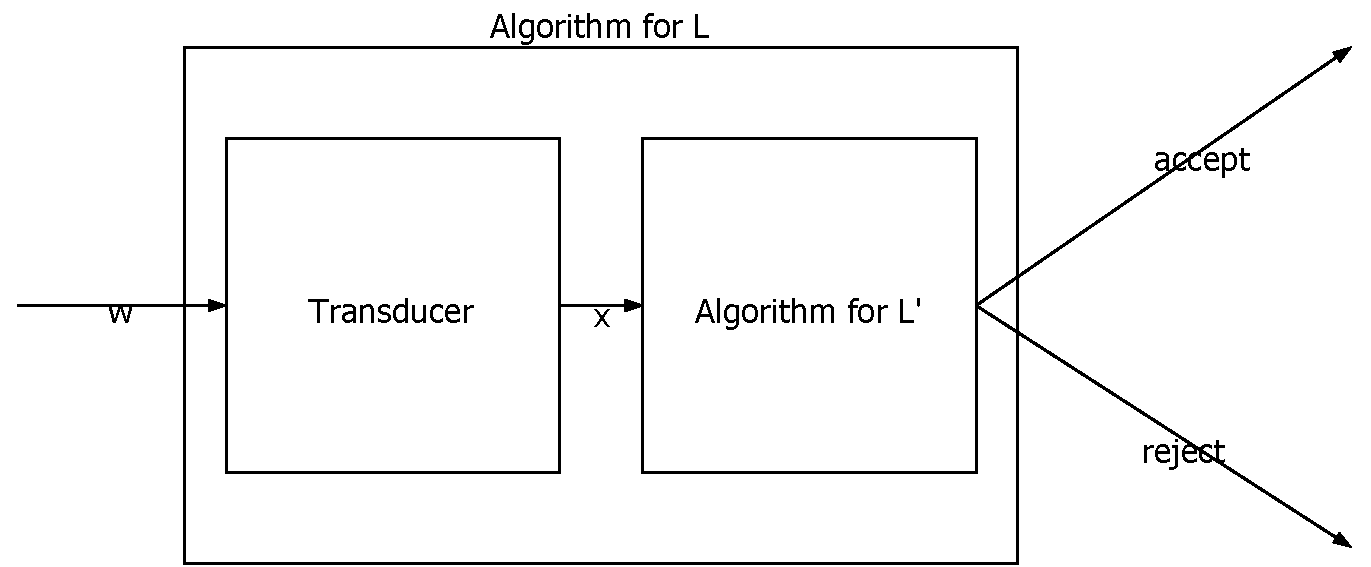
\includegraphics[scale=0.5]{Diagrams/Reduction}
\par\end{centering}
\caption{\label{fig:Reductions} The transducer serves as an adaptor for the
input string of $w$. It transforms $w$ into a string $x$which $L'$
can consume and produce an accept or reject decision. Algorithm $L'$
allows us to draw conclusions about the properties of $L.$}

\end{figure}


\subsection{Rice's Theorem}

We now need to prove the claim of Rice's Theorem: Every nontrivial
property $P$ of the Recursively Enumerable languages, $L_{P}$, is
undecidable. We\textquoteright re going to assume that the empty language
does not have property P. If that is not the case, then consider the
complement of P, say Q. Surely the empty language then has property
Q. But if we could prove that Q were undecidable, then P also must
be undecidable. That is, if L\_P were a recursive language, then so
would be L\_Q, since the class of recursive languages is closed under
complementation. We will use the UTM (i.e. $L_{U}$) obtained in Section\vref{subsec:haltingProblem}.
In this reduction we reduce $L_{U}$ to $L_{P}$. Because $L_{U}$
is undecidable this gives us the ability to say that $L_{P}$ is undecidable.
Our reduction must take the parameters $M$and $w$ and create a new
Turing Machine $M'$ such that $L(M')$ has property $P$ if and only
if $M$ accepts $w$. That is, the result of $M'$ is contingent on
the result of $M$'s result from taking in $w$. Our language property
testing machine $M'$ will be testing the language $L$ such that
$L$ is any language with a property $P$, and we let $M_{L}$ be
a TM that accepts $L$. $M'$ simulates $M$ on input $w$, and if
$M$ accepts $w$ then $M'$ simulates $M_{L}$ on the input $x$to
$M'$. $M'$ accepts its input $x$if and only if $M_{L}$ accepts
$x.$ Suppose $M$ accepts $w$, then $M'$will simulate $M_{L}$
on input $x$and therefore accepts $x$if and only if $x$is in $L.$
Formally, $L(M')=L(M_{L})=L$, the language of $M'$ is the language
of $M_{L}$, $L(M')$ has property $P$, and $M'$ is in $L_{P}.$
Now suppose the other case, $M$ does not accpet (never halts) $w$,
then $M'$ never starts the simulation of $M_{L}$ and thus never
accpets the input $x$, so $L(M')=L(M_{L})=\emptyset$. Therefore,
$L(M')$ does not have the property $P$. $M'$ is not in $L_{P}$.
This can viewed graphically in Figure\vref{fig:schematicRiceTheoremTM}.

\begin{figure}
\begin{centering}
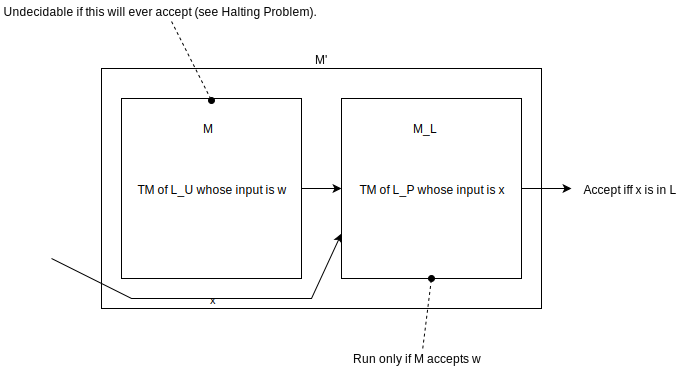
\includegraphics[scale=0.5]{Diagrams/riceTheoremTuringMachine}
\par\end{centering}
\caption{\label{fig:schematicRiceTheoremTM} Here we see a schematic of the
TM $M'$ in which the language of $M_{L}$ is the language $L_{P}$
who can only run once if $w$ is accepted by M whose language is $L_{U}$.
As a whole this can be regarded as a reduction from $L_{U}$ to $L_{P}$.
Since we know $L_{U}$ is undeciable then so is $L_{P}$. In essence
it is bootstrapped by $L_{U}$ undecidability. }

\end{figure}


\subsection{Post's Correspondence Problem}

Post's Correspondence Problem (PCP) will be a tool for us to use in
developing proving other problems are undecidable so its worth the
effort of understanding. PCP asks: Is there some some ordering of
indicies $i_{1}\ldots i_{k}$ for a list of cooresponding strings
$(w_{1},x_{1}),(w_{2},x_{2}),\ldots,(w_{n},x_{n})$ such that $w_{i}\ldots w_{n}=x_{i}\ldots x_{n}.$
A restriction we place on this question is that neither strings of
$w_{i}$ nor $x_{i}$ can be the empty string, and they share the
same alphabet. In less formal terms, PCP asks is there a way of concatenating
$w$-type strings with $x$-type strings so that they beome equivalent
strings. 

\subsection{PCP is Undecidable}

The proof that PCP is undeciable relies on two reductions. The first
reduction is from $L_{U}$, the language of the Univeral Turing Machine,
to $MPCP$. $MPCP$ can be regarded as a modified version of the PCP
problem such that the first pair must be chosen first when forming
the match on $w$ and $x.$ Then next reduction is from $MPCP$ to
$PCP$.

\subsubsection{Reduction from $L_{U}$ to MPCP}

//TODO

\subsubsection{Reduction from MPCP to PCP}

//TODO

\subsection{Some Real Problems}

//TODO

\part{Complexity}

\section{Time Complexity (Bachmann-Landau Notation)\label{sec:Big-O-Analysis}}

\section{Space Complexity}

\section{Intractable Problems}

In this section we learn about Time-Bounded Turing Machines, The Polynomial
Class of Problems, P, and the Exponenetial Class of Problems, NP.
Lastly we learn about Polynomial-Time Reductions. Refer to Michael
Garey and David Johnson's \emph{Computers and Intractability: A Guide
to the Theory of NP-Completeness }as a primary source for this subject
matter.

\subsection{Time Bounded Turing Machines}

We say a Turing machine is $T(n)$ time bounded, where$T(n)$ is some
function of $n$, like $n^{2}$ or $2^{n}$, if given an input of
length $n$, the machine always halts in at most $T(n)$ steps. 

\subsection{The Partial Order of Equivalance Classes P, NP, and NP-complete}

A Turing machine $M$ is said to be polynomial-time bounded if it
is time bounded by any polynomial. It could be linear, or quadratic,
or cubic, or $n^{1000}$, as long as it is some polynomial. The languages
who are said to be bounded by polynomial time make up the Polynomial
class P. For more complex polynomials you may wonder if they qualify
for the class P. A problem qualifies to be in P if it is less than
some polynomial. For example, $O(nlogn)$ is less than $O(n^{2})$,
and therefore it qualifies for the class P. The nondeterminitic polynomial
NP class of problems is defined in term of a NTM which has a polynomial
time nondeterministic algorithm. The algorithm should be composed
of two seperate states. Th first is the guessing stage, and the second
is the checking stage. A nondeterministic algorithm ``solves'' a
descisions problem $\Pi$ if the followung two properties hold for
all instances.
\begin{enumerate}
\item If the instance of the problem is an accepting instance, then there
exists \emph{some} structure $S$ that, when guessed for the input
of the instance, will lead to the checking stage to \emph{accept}
for the instance and $S$.
\item If the instance of the problem is an rejecting instance, then there
exists \emph{no} structure $S$ that, when guessed for the input of
the instance, will lead to the checking stage to \emph{reject} for
the instance and $S$.
\end{enumerate}
If there is a polynomial bound on the number steps an NTM must take
in any branch of its computation then the problem is in NP. The term
``complete problem'' for class of problems means that the problem
embodies the essence of all other problems in the class. Even though
it may appear that the problem doesn't. PCP embodies Turing Machine
computation. and the Knapsack Problem embodies all NTM computation.
Polynomial Time reductions allow us to define NP-Complete problems.
In order to show a problem $M$ to be NP-complete, we have to show
that every problem in NP is somehow embedded in $L$. We need a transformation
from every problem in NP to $M$, and this transformation has to be
sufficiently fast that if we had a deterministic polynomial time algorithm
for $M$, then we could use it to build a deterministic polynomial
time algorithm for each problem in NP. Formally, we say a problem
or language $M$ is NP-complete if, first of all, it is in NP, and
for every language $L$ in NP, there is a polytime reduction from
$L$ to $M$.

A final point on producing creating nondeterministic algorithms for
NP problems concerns the status of the algorithms complement. There
is a lack of symmetry the accepting and rejecting instances. \emph{In
a deterministic algorithm}, for a problem ``Given an instance of
the problem $I$, is $X$ true for $I$'', where $X$ is some property,
both the problem and its complement can be solved polynomially because
a deterministic algorithm always halts. To obtain the complent you
would just interchange the accepting and rejecting results. \emph{In
a nondeterministic algorithm},\emph{ }for example the complement of
the TSP problem\textendash this is not the case. Consider the complement
of TSP: ``Given a set of cities, intercity distances, and a bound
$B,$ is it true that \emph{no} tour of all the citeis has length
$B$or less? There is no know way to verify a ``yes'' answer to
this problem other than computing all possible tours (an exponential
algorithm). Thus membership P for a given problem implies membership
in coP. However membership in NP does not imply membership in coNP.
The prefix ``co'' implies the complement of this language class.
A tentative view of the world of NP can be seen in Figure\vref{fig:npHiearchy}.

\begin{figure}
\begin{centering}
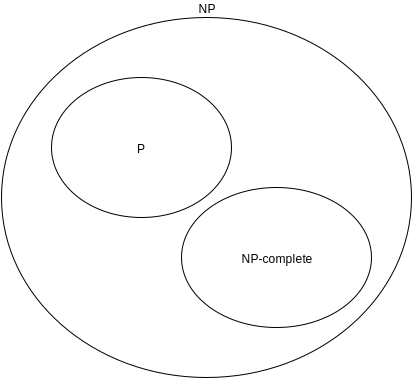
\includegraphics[scale=0.5]{Diagrams/npHierarchy}
\par\end{centering}
\caption{\label{fig:npHiearchy} This diagram gives a tentative view of the
membership relationship among the different language classes.}

\end{figure}


\subsection{Encoding Schemes}

It is important to note the effect an encoding scheme can have on
an algorithm. If the encoding scheme is poorly constructed the input
length might become exponential and thus violate one of the rules
of prooving NP-completeness. An example of reasonable encoding schemes
can be seen in in Figure\ref{fig:graphEncodingSchemes}. Similary,
if the output of our polynomial reduction becomes is not described
in a polynomial length of the input then it too violates the rules
of prooving NP-completeness. An example of this is a variant of the
Traveling Salesman Problem (TSP) problem. This variant gives a bounds
$B$ and asks for all tours of length $B$ or less yielding exponentially
many tours less than \textbf{$B$.} 
\begin{figure}
\begin{centering}
\begin{tabular}{|c|c|c|}
\hline 
Encoding Schemes & String & Length\tabularnewline
\hline 
Vertex list, Edge list & V{[}1{]}V{[}2{]}V{[}3{]}V{[}4{]}(V{[}1{]}V{[}2{]})(V{[}2{]}V{[}3{]}) & 36\tabularnewline
\hline 
Adjacency list & (V{[}2{]})(V{[}1{]}V{[}3{]})(V{[}2{]})() & 24\tabularnewline
\hline 
Adjacency matrix & 0100/1010/0010/0000 & 19\tabularnewline
\hline 
\end{tabular}
\par\end{centering}
\begin{centering}
\begin{tabular}{|c|c|}
\hline 
Lower Bound & Upper Bound\tabularnewline
\hline 
\hline 
$4v+10e$ & $4v+10e+(v+2e)\cdot\left\lceil \log_{10}v\right\rceil $\tabularnewline
\hline 
$2v+8e$ & $2v+8e+2e\cdot\left\lceil \log_{10}v\right\rceil $\tabularnewline
\hline 
$v^{2}+v-1$ & $v^{2}+v-1$\tabularnewline
\hline 
\end{tabular}
\par\end{centering}
\caption{\label{fig:graphEncodingSchemes} The table above demonstrates how
a graph's description can be described. The string length is given
by length column. For sparse graphs an adjaceny list representation
is beneficial. Dense graphs should be represented in an adjacency
matrix. The bounds describe the input length in terms of $v$ and
$e$, for $G(V,E)$ where $v=|V|$ and $e=|E|$. Graphs encoded in
any of these schemes will differ at most polynomially for any instance
of a graph.}

\end{figure}


\subsection{Transitivity of NP-completeness}

Polynomial transformations provide membership for languages to equivalence
classes with the following Lemma. Visually this can be seen in the
diagram for Figure\vref{fig:schematicRiceTheoremTM}.
\begin{lem}
If $L_{1}\propto L_{2}$ and $L_{1}$ $\epsilon$\emph{P, }then $L_{2}$
$\epsilon$\emph{P. }Equivalently, If $L_{1}\propto L_{2}$ and $L_{1}$
$\not\epsilon$\emph{ P, }then $L_{2}$ $\not\epsilon$\emph{ P.\label{lem:pMembership}}
\end{lem}
\begin{proof}
Let $\Sigma_{1}$and $\Sigma_{2}$ be the alphabets of languages $L_{1}$
and $L_{2}$ respectively, and let the function $f:\Sigma_{1}^{*}\rightarrow\Sigma_{2}^{*}$
be a \emph{polytime} function from $L_{1}$ to $L_{2}$. Let $M_{f}$
be a determinitic \emph{polytime} DTM recoginizer computing the function
$f$. Let $M_{2}$ be a \emph{polytime }DTM recognzier for $L_{2}.$
A \emph{polytime} recognizer for $L_{1}$ can be constructed by composing
$M_{f}$ and $M_{2}$. For an input $x$$\epsilon$ $L_{1}$ we first
apply the part of the program attributed to $M_{f}$ which yields
$f(x)$ $\epsilon$ $\Sigma_{2}$ ( a string of the $L_{2}$'s alphabet).
We the apply the recognizer $M_{2}$ to the program to determine if
the string $f(x)$ $\epsilon$$L_{2}.$ Since $x$$\epsilon$$L_{1}$
if and only if $f(x)$ $\epsilon$$L_{2}$ we now have a recognizer
for $L_{1}.$ The fact that this yields a polynomial algorithm is
derived from the fact that both $M_{f}$ and $M_{2}$ are polytime
algorithms themselves. 
\end{proof}
Reductions have the feature of transitivity. 
\begin{lem}
That is, if $L_{1}\propto L_{2}$ and $L_{2}\propto L_{3}$, then
$L_{1}\propto L_{3}$.\label{lem:reductionTransitiviy}
\end{lem}
\begin{proof}
Let $\Sigma_{1},\Sigma_{2},\Sigma_{3}$ be the alphabets for $L_{1},L_{2}$
and $L_{3}$ respectively. The function mapping the language of $L_{1}$
to the language of $L_{2}$ is given by $f_{1}:\Sigma_{1}^{*}\rightarrow\Sigma_{2}^{*}$,
and the function mapping the language of $L_{2}$ to the language
of $L_{3}$ is $f_{2}:\Sigma_{2}^{*}\rightarrow\Sigma_{3}^{*}$. Then
the function transforming the language of $L_{1}$ to the language
of $L_{3}$ is the composition of the given functions, $f(x)=f_{2}(f_{1}(x))$,
for all strings $x$in $L_{1}$. Clearly, $f(x)\epsilon L_{3}$ if
and only if $x\epsilon L_{1}$. The fact that $f$ can be computed
polynomially is derived from Lemma\vref{lem:pMembership}.
\end{proof}
An import lemma that allows us to constuct the NP-complete equivalence
class is the application of reduction transitivity to NP-complete
problems.
\begin{lem}
If $L_{1}$ and $L_{2}$ belong to NP, $L_{1}$ is NP-complete, and
$L_{1}\propto L_{2}$, then $L_{2}$ is NP-complete.
\end{lem}
\begin{proof}
Since $L_{2}$ $\epsilon$\emph{NP} all we need to do is show that,
for every $L'$\emph{ $\epsilon$ NP}, $L'\propto L_{2}$. Consider
any $L'$ $\epsilon$ \emph{NP}. Since $L_{1}$ is NP-complete, then
surely $L'\propto L_{1}$ by the definition of NP-completeness. The
tranistivity of $\propto$ seen in Lemma\vref{lem:reductionTransitiviy},
and the fact that $L_{1}\propto L_{2}$ implies that $L'\propto L_{2}$
. 

So it clear that once we have a single NP-complete problem to stand
in for $L_{1}$ it serves as a means to bootstrap the process of creating
the NP-complete equivalence class. The first NP-complete problem that
allows the process was provided by Steve Cook and is discussed in
Section\vref{subsec:Cook's-Theorem}.
\end{proof}

\subsection{Prooving NP-completeness}

In order to prove that a problem is NP-complete you will need to demonstrate
the following:
\begin{enumerate}
\item Show that the problem is in NP by giving a nondeterministic polytime
decider.
\item Select an known NP-complete problem.
\item Construct a transformation function $f$ from the NP-completer problem
to the problem in question.
\item Prove that the tranformation function $f$ is a polynomial tranformaton.
\end{enumerate}
Garey and Johnson suggest that three design patterns exist for proving
NP-completeness: restriction, local replacement and component design.
Descriptions of the three patters are given.

\subsubsection{Restriction}

\subsubsection{Local Replacement}

\subsubsection{Component Design}

\subsection{Polynomial Time Reductions}

Polynomial time transducers are TM's that take in an input of length
n, operate deterministically for some polynomial time $p(n)$. Produces
an output on a separate output tape, and the output must me at most
$p(n)$. Consider two languages or problems, say $L$ and $M$. We
say $L$ is polytime-reducible to $M$ if there is a polytime transducer
$T$ that takes an input $w$ that is an instance of $L$, produces
output $x$ that is an instance of $M$, and the answer to $L$ on
$w$ is the same as the answer to $M$ on $x$. That is, $w$ is in
$L$ if and only if $x$ is in $M$. 

Steve Cook and Dick Karp were the pioneers of NP-Completeness theory.
Cook concentrated on 3-SAT \textendash{} the question of whether an
expression of proposeitional logic was satisfiable, that is, made
true by some assignment of truth values to the propositional variables.
But shortly after Cook wrote his original paper on NP-completeness,
Dick Karp wrote another paper that showed many of the classical problems
that had been puzzling mathematicians, sometimes for centuries, were
NP-complete. Karp used only polytime reductions to the problem Cook
had proved NP-complete. Since then, it is generally accepted that
the preferred definition of NP-completeness is the one we gave here
\textendash{} the existence of polytime reductions. To make the distinction,
this notion of NP-completeness is often called Karp-completeness. 

\subsection{Cook-Levin Theorem\label{subsec:Cook's-Theorem}}

Recall from the Section\vref{sec:propositionalSententialLogic} on
propositional logic that we expresses the truth of expressions with
boolean operators. Expressions are built from two components variables
and constants using boolean the operators ($\land,\lor,\lnot).$ Constants
and the value of variables are either true (1) or false (0). The order
of precedence for the boolean operatios is NOT, AND, OR. The Satisfiability
Problem (SAT) is concened with determinig if there is a satisfying
assignment of boolean values to an expression such that the expression
is true. Instances of the SAT problem are represented with the parenthesis,
logical operators, and variables $x_{i}$ where $i$ is the $i^{th}$
binary integer. 

In order to prove that SAT is NP-Complete we must first show that
it is in NP. This can be done by giving an NTM that decides if an
instance of SAT of length $n$is satisfiable. The algorithm for this
Turing Machine can use nondeterminisc guessing to accomplish the goal.
First the NTM guesses truth values for the variables of the expression.
The NTM then checks the truth values of the expression. If the expression
is true, then accept, otherwise reject. We now know that SAT is in
NP.

The next step is to prove that SAT is NP-complete. Refer to Garey
and Johnson pg 39-44 for the indepth proof. Prior to reading this
you should understand Logic Programming \url{https://en.wikipedia.org/wiki/Logic_programming}
and Lambda Calculus \url{https://en.wikipedia.org/wiki/Lambda_calculus}.
At a high level the transformation function that they provide is based
on the idea that the intermediate descriptions of the Turing machine
can be translated into logical programming constraints which represent
the clauses of the satisfiability problem. 

\section{Specific NP-Complete Problems}

Garey and Johnson provide six additional foundational NP-complete
problems which they have found to be the most useful. The relationship
between these problems can be seen in Figure\vref{fig:npCompleteTree}. 
\begin{enumerate}
\item 3SAT asks the question: Is there a truth assignment for a set of clauses
in which all clauses have 3 variables? 
\item Three Dimmensional Matching asks the question: For the Cartesian product
of three disjount sets $X,Y,$ and $Z$, is there some subset of the
product that has unique coordinates for all members of the set? Formally,
$X\times Y\times Z$ = P, where the $|X|=|Y|=|Z|=q$, does there exists
a matching $M\subseteq P$ such that for all members of $M$ no coordiates
of the triple $(x_{i},y_{i},z_{i})$ are duplicated in any other element
of $M$, with $|M|=q$? That is, for M = \{$(x_{i},y_{i},z_{i})$
,$(x_{j},y_{j},z_{j}),$$\ldots,(x_{q},y_{q},z_{q})$\}, $x_{i}\neq x_{j}$,
$y_{i}\neq y_{j}$, and $z_{i}\neq z_{j}$. 
\item Vertex Cover asks the question: Is there a vertex cover for a given
graph $G$ of size $K$ or less? A vertex cover is a set of vertices
of a graph who are incident on edges which whose vertices make up
all the vertices of the graph. Formally, for a graph $G(V,E),$ is
there a vertex cover $V'\subseteq V$ such that $|V'|\leq K$, and
for each edge $\{u,v\}$ $\epsilon$ $E$ either $u$ or $v$ belong
to $V'$, but not both?
\item Clique asks the question: For a given graph $G(V,E)$ is there a strongly
connected component of size $J$ or more in $G$? A strongly connected
componenet is a set of vertices with a path between all pairs of vertices
(i.e. a complete subgraph)
\item .Hamiltonian Circuit asks the question: Is there a cycle in the graph
in which all vertices are visited only once? Formally, for a given
graph $G(V,E)$, with $V=\{v_{1},v_{2},\ldots v_{n}\}$, where n =
$|V|$. Is there an ordering of the members of $V$ such that $\{v_{1,}v_{n}\}$
$\epsilon$ $E$ and $\{v_{i},v_{i+1}\}$ $\epsilon$ $V$ for all
$i$, $1\leq i<n$?
\item Partition asks the question: Is there some way to evenly dividing
a set of elements such that the sum of their values is equivalent?
Formally, for a given set of elements $A=\{a_{1},a_{2},\ldots a_{n}\}$,
where $weight(a_{i})$ $\epsilon$$\mathbb{Z}^{+}$, is there a set
$A'\subseteq A$ such that:
\[
{\displaystyle \sum_{a\epsilon A'}weight(a)=\sum_{a\epsilon A-A'}weight(a)}
\]
\end{enumerate}
\begin{figure}
\begin{centering}
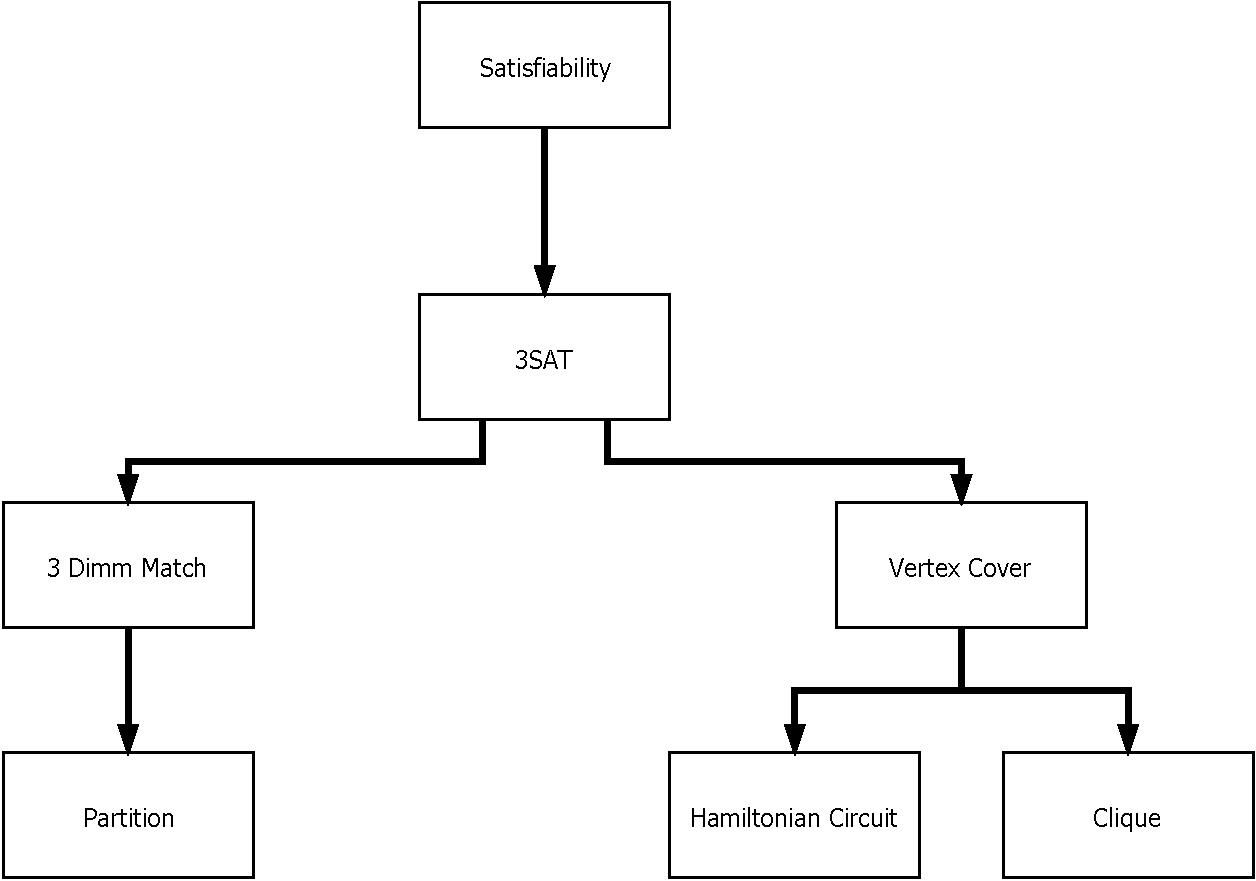
\includegraphics[scale=0.5]{Diagrams/npcompleteTree}
\par\end{centering}
\caption{\label{fig:npCompleteTree}This diagram depicts the hiearchy of the
NP-completeness proofs in this section.}

\end{figure}


\subsection{SAT to 3SAT}

\subsection{3SAT to 3DIMM Matching}

\subsection{3DIMM Matching to Partition}

\subsection{3SAT to Vertex Cover}

\subsection{Vertex Cover to Hamiltonian Circuit}

For the given graph G, the graph $G'$ can be generated to demonstrate
the equivalence of VC and HC. You can view both of these graphs in
Figure\vref{fig:vcToHC}.

\subsection{Vertex Cover to Clique}

\begin{figure}
\begin{centering}
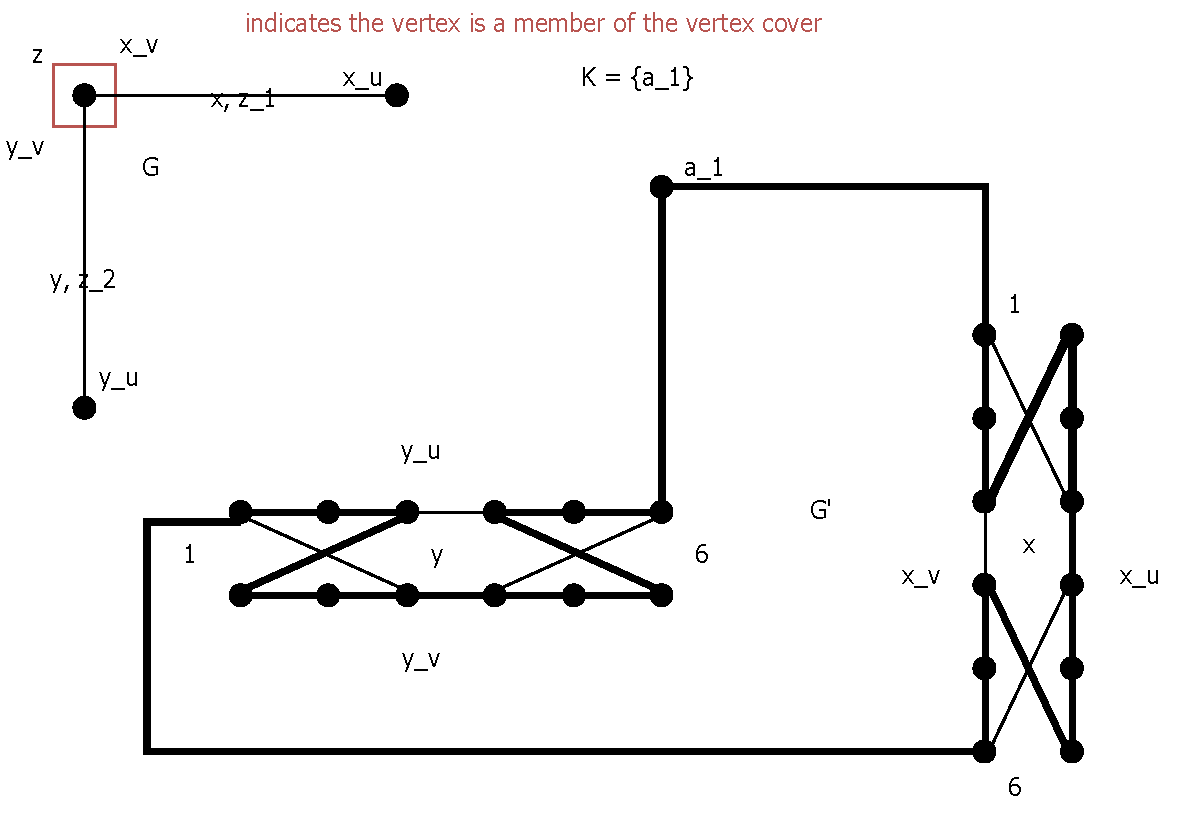
\includegraphics[scale=0.5]{Diagrams/vcToHC}
\par\end{centering}
\caption{\label{fig:vcToHC} A polynomial time mapping reduction from a graph
$G$ with a vertex cover of size $|K|$ allows us to generate a graph
$G'$ which has a Hamiltonian circuit. Here $K=\{a_{1}\}.$ }
\end{figure}


\part{Algorithms}

\section{Data Structures}

\subsection{Graphs}

\subsection{Trees}

\subsection{Lists}

\subsection{Queues}

\subsection{Arrays}

\section{Optimatility}

\section{Divide and Conquer}

T. Roughgardener lectures

\section{Greedy Algorithms}

\section{Approximation Algorithms\label{sec:Approximation-Algorithms}}

\subsection{Backtracking}

\subsection{Branch and Bound}

\subsection{Local Search}

\section{Randomized Algorithms\label{sec:Randomization-Algorithms}}

\subsection{Las Vegas and Monte Carlo}

\subsection{Game Theoretic Techniques}

\subsection{Moments and Deviations}

\subsection{Tail Inequalities}

\subsection{The Probablistic Method}

\section{Dynamic Programming\label{sec:Dynamic-Programming}}

\subsection{Recurrence Relations}

\subsection{Memoization}

\section{Fast Fourier Transform\label{sec:Fast-Fourier-Transform}}

\section{Shortest Path Algorithms}

\subsection{Dijkstra}

\subsection{Bellman-Ford}

\section{Maximum Flow\label{sec:Maximum-Flow}}

\subsection{Flows and Cuts}

\subsection{The Max-Flow Min-Cut Theorem}

\subsection{Flow Networks, Residual Networks, and Augmenting Flows}

\subsection{Ford-Fulkerson Algorithm}

\subsection{The Scaling Algorithm}

\subsection{Edmonds-Karp Algorithm}

\subsection{Dinic's Algorithm}

\section{Bipartite Matching\label{sec:Bipartite-Matching}}

\subsection{Nomencalture\textendash{} Matchings, Perfect Matchings, Maximum Matchings,
and Bipartiteness}

\subsection{The Frobenius-Hall Theorem}

\subsection{Hopcroft-Karp Algorithm}

\subsection{The Hungarian Algorithm}

\section{Appendix: Mathematical Rules}

This material will help you reason about various tasks including creating
inductive proofs and reasoning about Big O notation.

\subsection{Rules About Logarithms}

The logarithm $y=log_{b}x$ is equivalent to $x=b^{y}$. For example,
$log_{5}125=3$ and $5^{3}=125$. In this course and many other computer
science course the use of $log$ connotes $log_{2}$, where 2 is the
base of the logarithm.
\begin{center}
\begin{tabular}{cc}
$log_{b}b=1$ & $log_{b}1=0$\tabularnewline
$b^{log_{b}x}=x$ & $log_{b}(x^{r})=rlog_{b}x$\tabularnewline
$log_{b}b^{x}=x$ & $log_{b}\frac{x}{y}=log_{b}x-log_{b}y$\tabularnewline
$log_{b}(xy)=log_{b}x+log_{b}y$ & The domain of $log_{b}x$ is $x>0$\tabularnewline
\end{tabular}
\par\end{center}

\subsection{Rules About Exponents}
\begin{center}
\begin{tabular}{cc}
$a^{n}a^{m}=a^{n+m}$ & $\frac{a^{n}}{a^{m}}=a^{n-m}=\frac{1}{a^{m-n}}$\tabularnewline
$(a^{n})^{m}=a^{nm}$ & $a^{0}=1,a\neq0$\tabularnewline
$(ab)^{n}=a^{n}b^{n}$ & $(\frac{a}{b})^{n}=\frac{a^{n}}{b^{n}}$\tabularnewline
$a^{-n}=\frac{1}{a^{n}}$ & $\frac{1}{a^{-n}}=a^{n}$\tabularnewline
$(\frac{a}{b})^{-n}=(\frac{b}{a})^{n}=\frac{b^{n}}{a^{n}}$ & $a^{\frac{n}{m}}=(a^{\frac{1}{m}})^{n}=(a^{n})^{\frac{1}{m}}$\tabularnewline
\end{tabular}
\par\end{center}

\section{Appendix: Reference Material\label{sec:Appendix:-Reference-Material}}

The following sections provide some useful resources that will help
you along the way. 

\subsection{Software}
\begin{itemize}
\item Draw.io is a online tool for creating all sorts of diagrams. It will
be useful when creating automata.\url{https://www.draw.io}
\item LyX is a \LaTeX{} word processing application that will be useful
when drafting homework.\url{https://www.lyx.org}
\item Python is a useful programming language for experimenting with algorithms.
\url{https://www.python.org}
\item Mendeley is a good tool to organize your electronic library of books
and journal articles. \url{https://www.mendeley.com/}
\item Mathematica or MatLab to help your with linear programming \url{https://software.oit.gatech.edu}
\end{itemize}

\subsection{Books}

Even if you buy all these books it will not make you any better. I
strongly suggest you acquire these for free and purchase the ones
you find useful at a later date.
\begin{itemize}
\item \emph{How to Prove It: A Structured Approach} by Daniel J. Velleman
\url{https://amzn.com/0521675995}
\item \emph{Mathematical Reasoning: Writing and Proof} by Ted Sundstrom
\url{https://amzn.com/1500143413}
\item \emph{Book of Proof} by Richard Hammack \url{https://amzn.com/0989472108}
\item \emph{Understanding Analysis} by Stephen Abbot \url{https://amzn.com/1493927116}
\item \emph{Introduction to Probability} by Dimitri P. Bertsekas and John
N. Tsitsiklis \url{https://amzn.com/188652923X}
\item \emph{Discrete Mathematics and Its Applications} by Kenneth Rosen
\url{https://amzn.com/0073383090}
\item \emph{Introduction to the Theory of Computation} by Michael Sipser
\url{https://amzn.com/113318779X}
\item \emph{Introduction to Automata Theory, Languages and Computation}
by John Hopcroft, Rajeev Motwani and Jeffery Ullman \url{https://amzn.com/0321455363}
\item \emph{Computers and Intractability: A Guide to the Theory of NP-Completeness}
by Michael Garey and David Johnson \url{https://amzn.com/0716710455}
\item \emph{Algorithm Design} by Jon Kleinberg and Eva Tardos \url{https://amzn.com/0321295358}
\item \emph{Algorithms} by Sanjoy Dasgupta, Christos Papadimitriou, and
Vijay Vazirani \url{https://amzn.com/0073523402}
\item \emph{Introduction to Algorithms} by Thomas Cormen, Charles Leiserson,
Ronald Rivest, and Clifford Stein \url{https://amzn.com/0262033844}
\item \emph{Approximation Algorithms} by Vijay Vazirani \url{https://amzn.com/3540653678}
\item \emph{Randomized Algorithms} by Rajeev Motwani and Raghavan Prabhakar
\url{https://amzn.com/0521474655}
\item \emph{Linear Algebra and Its Applications }by David C. Lay \url{https://amzn.com/032198238X}
\item \emph{Linear and Nonlinear Programming} by David Luenberger and Ye
Yingyu \url{https://amzn.com/3319188410}
\end{itemize}

\subsection{Videos}
\begin{itemize}
\item Professor Harry Porter's YouTube playlist on the theory of computation.
\url{https://www.youtube.com/playlist?list=PLbtzT1TYeoMjNOGEiaRmm_vMIwUAidnQz}
\item Professor Tim Roughgardener's playlist on Logic \url{https://www.youtube.com/playlist?list=PLLH73N9cB21Xsgy39DP3xDqBN3lTaR8R5} 
\item Professor Tim Roughgardener's playlist on Data Structures and Algorithms
I \url{https://www.youtube.com/playlist?list=PLLH73N9cB21W1TZ6zz1dLkyIm50HylGyg} 
\item Professor Tim Roughgardener's playlist on Data Structures and Algorithms
II \url{https://www.youtube.com/playlist?list=PLLH73N9cB21VPj3H2xwTTye5TC8-UniA2}
\end{itemize}

\end{document}
